% latex4wp.tex		-*- LaTeX -*-
%
% LaTeX for Word Processor Users
% by Guido Gonzato, guido.gonzato (at) gmail.com
%
% This document was written with the Jed editor,
% http://www.jedsoft.org/jed, and the new LaTeX mode
% available from CTAN mirrors, e.g.
% http://www.ctan.org/tex-archive/support/jed
%
% Last updated: January 7, 2015

% debug
% \overfullrule=15pt

\documentclass[a4paper,11pt]{article}
\usepackage[margin=3cm]{geometry}
\usepackage{color}     % coloured stuff
\usepackage{ifpdf}     % ps/pdf output
\ifpdf
  \usepackage[pdftex]{graphicx}
  \pdfcompresslevel=9
\else
  \usepackage{graphicx}
\fi
\usepackage{alltt}     % like verbatim, but obeys LaTeX commands
\usepackage{dcolumn}   % aligning numbers to digital position
\usepackage{url}       % urls and links
\usepackage{colortbl}  % colour tables
\usepackage{pifont}    % dinglist
\usepackage{fancyvrb}  % fancy verbatim
\usepackage{boxedminipage} % what it says
\usepackage{framed}    % frames around stuff
\usepackage{rotating}  % rotate stuff
\usepackage[colorlinks,
            urlcolor=blue,
	    filecolor=magenta,
	    linkcolor=darkred,
	    hyperfootnotes=false]{hyperref} % browseable links
% \usepackage{fancyhdr}  % fancy headers and footers
\usepackage{marvosym}  % Euro sign and other nice characters
\usepackage[gen]{eurosym} % Euro sign
\usepackage{mflogo}    % Metafont logo
\usepackage{setspace}  % custom line spacing
\usepackage{tabularx}  % extended tabular environment
\usepackage{exa}       % local package for typesetting LaTeX examples
\usepackage{enumerate} % optional args for enumerate environment
\usepackage{wrapfig}   % wrapping text around figures
\usepackage[normalem]{ulem} % underline styles - !!! NOT IN MINT
\usepackage{slashbox}  % slashed box in tables - !!! NOT IN MINT
\usepackage{paralist}  % paragraph lists
\usepackage[version=3]{mhchem} % chemical formulae - !!! NOT IN MINT
\usepackage{lettrine}  % dropped capitals

\urlstyle{same} % urls in default font

% --- Definitions and new commands ---

\def\version {1.0.10}
\def\bs      {\textbackslash}
\def\unix    {\textsc{Unix}}
% \def\warning {\marginpar{\Huge{\textcolor{red}{\Stopsign}}}}
\def\note    {\marginpar{\Huge{\textcolor{magenta}{\Writinghand}}}}
\def\PS      {\textsc{PostScript}}
\definecolor {darkred}{rgb}{0.75,0,0}

\hyphenation{lo-cal-tex-mf land-sca-pe}

\newcounter{fnsym}
\setcounter{fnsym}{1}
%\newcounter{tmpbaselineskip}
%\setlength{tmpbaselineskip}{\value{\baselineskip}}

\newenvironment{margins}[2]
{ 
  \begin{list}{} {
    \setlength{\leftmargin}{#1}
    \setlength{\rightmargin}{#2}
  } \item }
{\end{list}}

\newenvironment{warn}
{ % beg def
  \medskip
  \begin{minipage}[t]{0.1\linewidth}
    \vspace{0pt}
    \textcolor{magenta}{\Huge{\Pointinghand}}
  \end{minipage}%
  \begin{minipage}[t]{0.88\textwidth}
    \vspace{0pt}
    \begin{small}
      \begin{spacing}{0.97}
}
{ % end def
      \end{spacing}
    \end{small}
  \end{minipage}
  \medskip
}

\newcommand{\package}[1]
{\textsf{#1}}

\newcommand{\parm}[1]
{\texttt{#1}}

\newcommand{\cmdparm}[1]
{\textit{#1}}

\newcommand{\env}[1]
{\texttt{#1}}

\newcommand{\cmd}[1]
{\texttt{\bs{}#1}}

\newcommand{\cmdline}[1]
{\texttt{#1}}

\newcommand{\menu}[1]
{\textsf{#1}}

\newcommand{\entry}[2]
{\textsf{#1/#2}}

\newcommand{\app}[1]
{\texttt{#1}}

\newcommand{\file}[1]
{\texttt{#1}}

\newcommand{\style}[1]
{\texttt{#1}}

\newcommand{\ltx}[1]
{\texttt{#1}}

% --- end of definitions and new commands ---
% ok, let's start

\begin{document}

\pagenumbering{roman}
\setlength{\parindent}{0pt}
\setlength{\parskip}{3pt}

\title{\LaTeX{} for Word Processor Users\\version \version}

\author{Guido Gonzato, Ph.D.\\
\texttt{guido.gonzato@gmail.com}}

% I want to use the dagger sign as footnote symbol
\renewcommand{\thefootnote}{\fnsymbol{footnote}}
\setcounter{footnote}{2}

\date{\today}

% let's put things back to normal
\renewcommand{\thefootnote}{\arabic{footnote}}
\setcounter{footnote}{1}

\maketitle

\begin{abstract}

  Text processing with \LaTeX{} offers several advantages over word
  processing. However, beginners may find it hard to figure out how to
  perform common tasks and obtain certain features. This manual
  attempts to ease the transition by drawing comparisons between word
  processing and \LaTeX{} typesetting. The main word processor
  capabilities are listed, along with their equivalent \LaTeX{}
  commands. Many examples are provided.

\end{abstract}

\begin{footnotesize}
  \tableofcontents
  \listoftables
  \listoffigures
\end{footnotesize}

% INTRODUCTION

% \pagestyle{fancy}
\pagenumbering{arabic}

\section{Introduction}

First of all, let me state that this is \emph{not} a \LaTeX{} primer!
If you're reading this document, I assume that you have at least a
basic understanding of \LaTeX{} and of its basic commands. In this
guide, I'll explain how to replace a word processor effectively using
\LaTeX.

Word processors are the `killer app' in modern office automation.
They're perceived to be easier than \LaTeX{} as they have a friendly
WYSIWYG interface, and the average secretary will learn to use them in
a relatively short time. The problem is, these beasts keep growing
slow, bloated,\footnote{once upon a time, I wrote my thesis on a 128k
RAM, Z80-based home computer. The word processor WordStar and my
thesis fit on a single CP/M-bootable 720K floppy, with lots of room to
spare!} buggy, crash-prone, expensive, virus ridden, and incompatible
with each other. Not to talk about their default output quality.

\LaTeX{} is an excellent alternative (in some cases, it is the
\emph{only} viable alternative); but it's not much intuitive for those
accustomed to WYSIWYG.

To sum up, sometimes you may want to use word processor-like
features---but using \LaTeX. It would be nice to know how to obtain
some effects with \LaTeX{} when you know how to get them with your
once-favourite \texttt{:-)} word processor.

That's why I wrote this quick reference. As I said, it assumes some
basic \LaTeX{} knowledge; if it's not the case, I suggest that you go
to \url{http://www.ctan.org/starter.html} and download 
\href{http://www.ctan.org/tex-archive/info/lshort/}{The (Not So) Short
Introduction to \LaTeX2e{}}. Another good primer is
\url{http://en.wikibooks.org/wiki/LaTeX/}.

In the following sections, we shall navigate through the menus and
menu items of an imaginary word processor, finding out the
corresponding \LaTeX{} way of doing the same work.

% -----

% WP WITH LATEX

\subsection{Preliminaries}

Many word processor features are implemented by the editor; others by
standard \LaTeX{} commands; others still are obtained using
\emph{packages}. These are sets of macros that extend \LaTeX{}
providing new commands and environments. There are lots of packages
around: the only problem is knowing where they are, what they do, and
how to install them. More about packages in
Section~\ref{sec:packages}.

Packages and other \TeX{}-related material are available at many sites
that constitute the CTAN: the Comprehensive TeX Archive Network. I
already mentioned \url{http://www.ctan.org}; this site has a wide list
of mirrors. From now on, \href{http://www.ctan.org}{CTAN:} means `your
favourite CTAN mirror here, starting from the \TeX{} directory'. For
instance, you can get \LaTeX{} for your platform from
\href{http://www.tex.ac.uk/tex-archive/systems}{CTAN://systems} (e.g.,
\url{http://www.tex.ac.uk/tex-archive/systems/}).

To write your documents, you will need a good text editor. A better
choice for beginners is a \emph{\LaTeX{} IDE}: an editor dedicated
to writing \LaTeX{} source, with preview and many facilities.

I suggest that you install one of the programs listed below; all of
them are Free/Open Source software.

\begin{itemize}

  \item Texmaker (multiplatform):\\
  \url{http://www.xm1math.net/texmaker/index.html}

  \item TeXstudio (multiplatform):\\
  \url{http://texstudio.sourceforge.net/}

  \item TeXworks (multiplatform):\\
  \url{http://tug.org/texworks/}
  
%  \item LyX, an almost-WYSIWYG \LaTeX{} editor (multiplatform):\\
%  \url{http://www.lyx.org/}
  
  \item TeXShop (Mac OS X):\\
  \url{http://www.uoregon.edu/~koch/texshop/}
  
  \item TeXnicCenter (Windows):\\
  \url{http://www.texniccenter.org/}
    
\end{itemize}

Information about \LaTeX{} on the Mac can be found at
\url{http://www.esm.psu.edu/mac-tex/}.

% -----

% EDITOR-SUPPORTED

\subsubsection{Editor-Supported Features}

\LaTeX{} is just a formatter: things like cut and paste, search and
replace etc. are delegated to the editor. Table~\ref{tab:editing}
summarises the main commands of popular editors for geeks: GNU
\app{emacs} and \app{vim} with their native key bindings, and
\app{jed} configured for Borland IDE key bindings.

\begin{table}[htbp]
\begin{center}
\begin{tabular}{|lccc|} \hline
\textbf{Action} & \textbf{Emacs} & \textbf{Vim} & \textbf{Jed} \\
\hline
command mode & \texttt{Alt-X} & \texttt{ESC} & \texttt{Alt-X} \\
insert mode & n/a & \texttt{i a o O} & n/a \\
line editor mode & n/a & \texttt{:} & n/a \\
%\hline
\multicolumn{4}{|c|}{\textit{\rule{0pt}{0.3cm}file operations}} \\
%\hline
open file & \texttt{Ctrl-X Ctrl-F} & \texttt{:e} & \texttt{Ctrl-KE}\\
insert file & \texttt{Ctrl-Xi} & \texttt{:r} & \texttt{Ctrl-KR}\\
save file & \texttt{Ctrl-X Ctrl-S} & \texttt{:w} & \texttt{Ctrl-KD}\\
save as & \texttt{Ctrl-X Ctrl-W name} & \texttt{:w name} & \texttt{Ctrl-KS}\\
close file & \texttt{Ctrl-XK} & \texttt{:q} & \texttt{Ctrl-KQ}\\
change buffer & \texttt{Ctrl-XB} & \texttt{bN} & \texttt{Ctrl-KN}\\
undo & \texttt{Ctrl-XU} & \texttt{u} & \texttt{Ctrl-U}\\
redo & \texttt{Ctrl-\^} & \texttt{Ctrl-R} & \texttt{Ctrl-G Ctrl-U}\\
exit & \texttt{Ctrl-X Ctrl-C} & \texttt{:qa!} & \texttt{Ctrl-KX}\\
%\hline
\multicolumn{4}{|c|}{\textit{\rule{0pt}{0.3cm}moving around}}\\
%\hline
word left & \texttt{Alt-B} & \texttt{b} & \texttt{Ctrl-A}\\
word right & \texttt{Alt-F} & \texttt{w} & \texttt{Ctrl-F}\\
start of line & \texttt{Ctrl-A} & \texttt{0} & \texttt{Ctrl-QS}\\
end of line & \texttt{Ctrl-E} & \texttt{\$} & \texttt{Ctrl-QD}\\
page up & \texttt{Alt-V} & \texttt{Ctrl-U} & \texttt{Ctrl-R}\\
page down & \texttt{Ctrl-V} & \texttt{Ctrl-D} & \texttt{Ctrl-C}\\
start of buffer & \texttt{Alt-<} & \texttt{1G} & \texttt{Ctrl-QR}\\
end of buffer & \texttt{Alt->} & \texttt{G} & \texttt{Ctrl-QC}\\
line n. & \texttt{Alt-G n.} & \texttt{n.G} & \texttt{Ctrl-QI}\\
%\hline
\multicolumn{4}{|c|}{\textit{\rule{0pt}{0.3cm}deleting}}\\
%\hline
character left & \texttt{Ctrl-H} & \texttt{X} & \texttt{BS}\\
character right & \texttt{Ctrl-D} & \texttt{x} & \texttt{Alt-G}\\
word left & \texttt{Alt-DEL} & \texttt{db} & \texttt{Alt-BS}\\
word right & \texttt{Alt-D} & \texttt{dw} &\texttt{Ctrl-T} \\
end of line & \texttt{Ctrl-K} & \texttt{d\$} & \texttt{Ctrl-QY} \\
line & \texttt{Ctrl-A Ctrl-K} & \texttt{dd} & \texttt{Ctrl-Y} \\
%\hline
\multicolumn{4}{|c|}{\textit{\rule{0pt}{0.3cm}search \& replace}}\\
%\hline
search & \texttt{Ctrl-S text} & \texttt{/text} & \texttt{Ctrl-QS}\\
replace & \texttt{Alt-\%} & \texttt{:s/old/new/g} & \texttt{Ctrl-QA}\\
%\hline
\multicolumn{4}{|c|}{\textit{\rule{0pt}{0.3cm}blocks}}\\
%\hline
start selection & \texttt{Ctrl-SPACE} & \texttt{v} & \texttt{Ctrl-KB} \\
cut & \texttt{Ctrl-W} & \texttt{D} & \texttt{Ctrl-KY} \\
copy & \texttt{Alt-W} & \texttt{Y} & \texttt{Ctrl-KH} \\
paste & \texttt{Ctrl-Y} & \texttt{P} & \texttt{Ctrl-KC} \\
\hline
\end{tabular}
\caption{Useful key bindings for Emacs, Vim, and Jed in IDE mode.}
\label{tab:editing}
\end{center}
\end{table}

% -----

% ADDING PACKAGES

\subsubsection{Adding Packages}
\label{sec:packages}

The following information applies to \app{TeX Live}, which ships with
most GNU/Linux distributions. It may also work on MacTeX, but I have
no first-hand experience. Instructions for MiK\TeX{} (probably the
most popular implementation for Windows) will follow below.

A large collection of \LaTeX{} packages is natively supported; for
instance, Ubuntu provides lots of \app{texlive-*} packages. Please
note the ambiguity: we're talking of \texttt{.deb} \emph{packages}
containing \LaTeX{} \emph{packages}.

If you need to install an unsupported package, do the following.

\begin{enumerate}

  \item create this directory structure:
  
  \begin{verbatim}
  $ mkdir -p ~/texmf/tex/latex
  \end{verbatim}
  
  Under this directory, new packages will be installed.

  \item get the package (typically as a zip-compressed directory) from
  your favourite CTAN mirror; let's call it \app{foo.zip}
  
  \item unpack it in the right place:
  
  \begin{verbatim}
  $ mkdir ~/texmf/tex/latex/foo
  $ mv foo.zip ~/texmf/tex/latex/foo
  $ cd ~/texmf/tex/latex/foo ; unzip foo.zip
  \end{verbatim}
 
  \item If no \texttt{.sty} file exists, run the command
  \texttt{latex foo.ins} or \texttt{latex foo.dtx} to create it;
  
  \item run the command \cmdline{texhash \~{}/texmf}.
    
\end{enumerate}

To add a package to MiK\TeX, create the directory
\path{\latex\newpackage} under \path{C:\localtexmf\tex\} and put the
relevant files in there. Proceed as above, then run MiKTeX Options and
click on the `Refresh now' button. Alternatively, issue the command
\cmdline{initexmf -u}. That's it!

Once a package is installed, you make it available in your documents
adding a line under the \texttt{documentclass} declaration:

\begin{verbatim}
\usepackage{foo}
\end{verbatim}

% -----

\subsubsection{Adding the Info Page}
\label{sec:infopage}

`Man' and `Info' pages are command-line sources of documentation for
software, widely employed in \unix{} and Linux systems. If your
\LaTeX{} distributions lacks the \file{latex2e.info} info page, do the
following:

\begin{enumerate}
  
  \item download it from
  \url{http://tug.ctan.org/info/latex2e-help-texinfo/latex2e.info};
  
  \item run these commands:
  
  \begin{verbatim}
  $ sudo cp latex2e.info /usr/share/info/
  $ sudo ginstall-info latex2e.info dir
  \end{verbatim}
   
\end{enumerate}

Now, \cmdline{info latex} or \cmdline{info latex2e} is available.

% -----

% GOLDEN RULES

\subsection{The Golden Rules}

Before we start, please keep this in mind:

\begin{enumerate}

  \item get used to \emph{structuring} your documents: think in terms of
  parts, chapters, sections, and so on. This holds true even if you're
  not writing a scientific paper.

  \item \LaTeX{} explicitly discourages the user from messing about with
  formatting parameters. Don't worry too much about the \emph{looks}
  of what you're writing, concentrate on the \emph{contents}.

\end{enumerate}

Applying these simple rules, your printed material will magically look
professional.

That said, this guide (which breaks the second rule somehow!) will
help you overcome the second rule. So, you will also be able to
compose unstructured material such as circulars, notices, poster, etc.


\bigskip
{\color{blue} \dingline{45}}

% -----

% FILE

\section{The \menu{File} Menu}

Obviously, some entries of this menu have nothing to do with \LaTeX{}:
\entry{File}{Open}, \entry{File}{Save}, \entry{File}{Close} depend on
the editor. 

% -----

% FILE/NEW

\subsection{\entry{File}{New}}
\label{sec:filenew}

This is the \LaTeX{} equivalent of a blank page:

\begin{Verbatim}[fontsize=\small]
\documentclass{article}
\thispagestyle{empty} % no page number
\begin{document}
% This is a comment. Write your stuff here.
\end{document}
\end{Verbatim}

As documents written in \LaTeX{} are inherently structured, this is a
more realistic example:

\begin{Verbatim}[fontsize=\small]
\documentclass[a4paper,12pt]{article}
\begin{document}
\title{My Document}
\author{John Smith}
\date{London, \today}
\maketitle
\begin{abstract}
This is a very short article.
\end{abstract}
\tableofcontents
\listoftables
\listoffigures
\section{First Section}
\label{sec:start}
This is the text of the section. See \cite{Gonzato} for details.
\section{End}
\label{sec:end}
This is the end of the document. Please go to Section
\ref{sec:start} to read it again.
\begin{thebibliography}{99}
\bibitem{Gonzato} Gonzato G. \textit{\LaTeX{} for Word Processor
Users}. CTAN, 2001--2015.
\end{thebibliography}
\end{document}
\end{Verbatim}

More document templates are listed in Appendix~\ref{ap:templates}.

% -----

% FILE/SAVE AS

\subsection{\entry{File}{Save As{\ldots}}}

The following tools are handy if you want to convert \LaTeX{} to other
formats:

\begin{itemize}

  \item \app{\TeX4ht} is probably the best \LaTeX{} to HTML converter:\\
  \url{http://tug.org/tex4ht}

  \item \app{latex2html}, another converter to HTML:\\
    \url{http://saftsack.fs.uni-bayreuth.de/~latex2ht/},\\
    \href{http://www.ctan.org/tex-archive/support/latex2html}
    {CTAN://support/latex2html}
    
  \item \app{latex2rtf}, a converter to Rich Text Format:\\
  \href{http://www.ctan.org/tex-archive/support/latex2rtf}
  {CTAN://support/latex2rtf}

  \item \app{detex} (a command line converter) removes all \LaTeX{} tags and
  outputs plain text:\\
  \url{http://www.cs.purdue.edu/homes/trinkle/detex/}, \\
  \href{http://www.ctan.org/tex-archive/support/detex}
  {CTAN://support/detex/}

  
\end{itemize}

See also Section~\ref{sec:prpreview} for details on PDF creation.

% -----

% FILE/SAVE AS TEMPLATE

\subsection{\entry{File}{Save As Template}}

Saving a \LaTeX{} `template' would mean, as I see it, create a new
\LaTeX{} package. This is complex matter that goes beyond the scopes
of this guide.

% -----

% FILE/IMPORT

\subsection{\entry{File}{Import}}

These tools convert from other formats to \LaTeX{}:

\begin{itemize}

  \item \app{rtf2latex}: 
  \href{http://www.ctan.org/tex-archive/support/rtf2latex}
  {CTAN://support/rtf2latex}
  
  \item \app{html2latex}: 
  \href{http://www.ctan.org/tex-archive/support/html2latex}
  {CTAN://support/html2latex}
  
  \item \app{wvware} is a set of tools that convert from MS Word to
  several formats including \LaTeX{};
  \url{http://wvware.sourceforge.net}
  
  \item the free word processor Abiword, \url{http://www.abiword.org},
  imports MS Word and can export \LaTeX.
  
  \item \app{txt2tex}: 
  \href{http://www.ctan.org/tex-archive/support/txt2tex}
  {CTAN://support/txt2tex} does a fairly good job at converting plain
  text files into \LaTeX.
  
\end{itemize}

Other \texttt{*2latex} converters are available at the same address.

Another interesting extension is OOoLatex, a set of macros for
OpenOffice: \url{http://ooolatex.sourceforge.net/}. Libreoffice users
have an equivalent extension called TexMaths,
\url{http://roland65.free.fr/texmaths/}.


% -----

% FILE/PAGE SETUP

\subsection{\entry{File}{Page Setup}}
\label{sec:pagesetup}

The normal method for setting paper size, orientation, and margins, is
to use parameters in \cmd{documentclass}. Paper size can be
\parm{a4paper}, \parm{a5paper}, \parm{b5paper}, \parm{letterpaper},
\parm{legalpaper}, \parm{executivepaper}; orientation is
\parm{portrait} by default, or optionally \parm{landscape}. For
example, 

\begin{Verbatim}[fontsize=\small]
\documentclass[a5paper,landscape,12pt]{article}
\end{Verbatim}

Document-wide margins are set with the \cmd{setlength} command, which
is used to change the value of variables and counters:

\begin{Verbatim}[fontsize=\small]
\setlength{\leftmargin}{2cm}
\setlength{\rightmargin}{2cm}
\setlength{\oddsidemargin}{2cm}
\setlength{\evensidemargin}{2cm}
\setlength{\topmargin}{-1cm}
\setlength{\textwidth}{18cm}
\setlength{\textheight}{25cm}
\end{Verbatim}

The \package{geometry} package allows for complete control of
parameters such as paper size, margins width, and so on.
\package{geometry} has far too many options to list them all, and
you're invited to read its documentation. A fairly complete example of
its usage is shown below. In this example, some parameters are not
compatible with each other, and are there for purpose of argument
only.

\begin{Verbatim}[fontsize=\small]
\usepackage{geometry}  % top of document
...
\geometry{paperwidth=25cm}
\geometry{paperheight=35cm}
% or: \geometry{papersize={25cm,35cm}}
\geometry{width=20cm}  % total width
\geometry{heigth=30cm} % total heigth
% or: \geometry{total={20cm,30cm}}
\geometry{textwidth=18cm}  % width - marginpar
\geometry{textheight=25cm} % heigth - header - footer
% or: \geometry{body={18cm,25cm}}
\geometry{left=3cm}    % left margin
\geometry{right=1.5cm} % right margin
% or: \geometry{hmargin={3cm,2cm}}
\geometry{top=2cm}     % top margin
\geometry{bottom=3cm}  % bottom margin
% or: \geometry{vmargin={2cm,3cm}}
\geometry{marginparwidth=2cm}
\geometry{head=1cm}    % header space
\end{Verbatim}

Options can also be set this way:

\begin{Verbatim}[fontsize=\small]
\usepackage[left=3cm, right=2cm]{geometry}
\end{Verbatim}

% -----

% FILE/PAGE SETUP/HEADERS AND FOOTERS

\subsubsection{\entry{Page Setup}{Headers and Footers}}
\label{sec:headers_footers}

The \package{fancyhdr} package provides the new command
\cmd{pagestyle\{fancy\}}. This will create a header reporting the
current section (\style{chapter} in \style{book.cls}) and subsection,
and a footer with the page number: pretty fancy indeed. Headers and
footers can obviously be customised. They are made of three parts: a
left-aligned part, a centre-aligned part, and a right-aligned part. To
set those, use the commands like in this example:

\begin{Verbatim}[fontsize=\small]
\usepackage{fancyhdr}
...
\lhead{} % empty
\chead{Hello, world!}
\rhead{Page \thepage} % page number
\lfoot{}              
\cfoot{\textbf{Hello!}}
\rfoot{}
\end{Verbatim}

% -----

% FILE/PRINTER SETUP

\subsection{\entry{File}{Printer Setup}}

This is highly OS-dependent, and definitely outside of the scopes of
\LaTeX{}. Assuming that you're using a \unix-like system, these tips
may come in handy:

\begin{itemize}

  \item \cmdline{lpr -P printername} prints to the specified printer;
  
  \item \cmdline{lpr -\# 10} prints 10 copies;
  
  \item \cmdline{lpr -r} removes the file after printing it

\end{itemize}

See below for more tips.

% -----

% FILE/PRINT PREVIEW

\subsection{\entry{File}{Print Preview}}
\label{sec:prpreview}

When the \LaTeX{} input file is ready, you have several options:

\begin{itemize}

  \item convert it to \file{.dvi} (\cmdline{latex file.tex}) and previewing
    it with \app{xdvi}, \app{yap} or other DVI previewer;
    
  \item convert the \file{.dvi} to \PS{} with \app{dvips}, then use
    some variant of \app{Ghostview};
    
  \item producing a \file{.pdf} file with \app{dvipdf} or directly
  with \app{pdflatex}.
  
\end{itemize}

In my opinion, producing a \file{.pdf} file is the best option, as it
makes for widest portability.

While \app{dvipdf} is just a script that converts the \file{.dvi} to
\file{.ps} then to \file{.pdf}, using \app{pdflatex} is more
interesting. In fact, some packages like \package{hyperref} and
\package{url} make the resulting \file{.pdf} file browseable; see
Section~\ref{sec:hyperlink}. However, \note{} using \app{pdflatex} you
might experience problems with other packages. More details in
Section~\ref{sec:figure}.

% -----

% FILE/PRINT

\subsection{\entry{File}{Print}}

Simply use \cmdline{lpr file.ps} from the command line, or via the
\entry{File}{Print} menu entry of your previewer.

% -----

% FILE/VERSIONS

\subsection{\entry{File}{Versions}}

Although the \package{version} package provides basic facilities for
versioning \LaTeX{} sources, using external tools is usually a better
choice.

There are lots of programs for revision control and collaborative
writing. While old-style geeks may want to use a single-user tool like
RCS (I do), more powerful and multi-user tools like Subversion, Git,
Mercurial etc.\ may be preferable. Some of them are integrated with
the editor.

An introduction to \LaTeX{} and Subversion is here:\\
\url{http://tug.org/pracjourn/2007-3/kalderon-svnmulti/}.

% -----

% EDIT

\section{The \menu{Edit} Menu}

This menu has more to do with the editor than \LaTeX{} features. To
begin with, refer to Table~\ref{tab:editing} that shows the key
bindings for the entries \entry{Edit}{Cut}, \entry{Edit}{Copy},
\entry{Edit}{Paste}, \entry{Edit}{Find}, and \entry{Edit}{Replace} of
some common editors.

Selecting text is not only performed for subsequent cut and paste, but
also for applying styles to the selected text. The equivalent action
in \LaTeX{} is to enclose the text either between braces, or in an
environment. For example, to apply the bold attribute to a portion of
text you will use one of the following:

\begin{example}
this is \textbf{bold text;}\\
this is also
{\bfseries bold text;}\\
\begin{bfseries}
this is bold text, too!
\end{bfseries}
\end{example}

% -----

% EDIT/AUTOTEXT

\subsection{\entry{Edit}{Autotext}}

We call \emph{autotext} the feature that makes you type, say, `PS' to
have the word `PostScript' automatically expanded. This is an editor
feature, but there's a rough \LaTeX{} equivalent:

\begin{Verbatim}[fontsize=\small]
\def\PS    {\textsc{PostScript}}
\end{Verbatim}

which will insert the equivalent of \verb|\textsc{PostScript}|
whenever you type \verb|\PS|. Beware, case is important.

% -----

% INSERT

\section{The \menu{Insert} Menu}
\label{sec:menu_insert}

% -----

% INSERT/BREAKS

\subsection{\entry{Insert}{Breaks}}

\begin{itemize}

  \item a non-breakable space is set with \textasciitilde{} (tilde)
  
  \item to force a line break, use \cmd{linebreak} or \cmd{newline};
  see below for details
  
  \item to start a new paragraph use a blank line, or \cmd{\bs} (possibly
  followed by an optional space, as in \cmd{\bs[1cm]}), or \cmd{par}
  
  \item finally, for a page break use \cmd{newpage} or \cmd{clearpage}
  
\end{itemize}

Unlike \cmd{newline}, \cmd{linebreak} stretches the line to the
margins:

\begin{example}
I am stretched!\linebreak
But I am not.\newline
Ok, now you get it.
\end{example}

Besides, \cmd{clearpage} differs from \cmd{newpage} in that it prints
all pending \emph{floats}, that is figures and tables. Floats will be
explained in Section~\ref{sec:figure}.

% -----

% INSERT/ENUMERATED LIST

\subsection{\entry{Insert}{Enumerated List}}

Bulleted and enumerated lists correspond to the \env{itemize} and
\env{enumerate} environments. To customise the bullet in a list
environment, you can specify it as an argument to \cmd{item}:

\begin{example}
\begin{itemize}
  \item[*] with an asterisk;
  \item[-] with a dash;
  \item[.] with a dot.
\end{itemize}
\end{example}

Another way is to redefine the style of the
\emph{counters}\footnote{each text element numbered by \LaTeX{}
(sections, lists, figures, etc.) has a counter associated with it.}
hat refer to the digits in the first- to fourth-level lists. These
counters are \cmd{labelitemi}, \cmd{labelitemii}, \cmd{labelitemiii}
and \cmd{labelitemiv} for itemised lists; \cmd{labelenumi},
\cmd{labelenumii}, \cmd{labelenumiii} and \cmd{labelenumiv} for
enumerated lists.

There are several styles: \cmd{arabic} for `normal' numbers,
\cmd{roman} for lower-case roman numerals (e.g., viii is 8),
\cmd{Roman} for upper-case roman numerals, \cmd{alph} and \cmd{Alph}
for lower- and upper-case letters, and \cmd{fnsymbol} that I will not
explain for now:

\begin{example}
\begin{itemize}
\renewcommand{\labelitemi}{*}
\renewcommand{\labelitemii}{-}
  \item first level, item 1
  \item first level, item 2
  \begin{itemize}
    \item second level, item 1
    \item second level, item 2
  \end{itemize}
  \item first level, item 3
\end{itemize}
\end{example}

To use, say, roman numbers and uppercase letters in enumerated lists,
do this:

\begin{example}
\begin{enumerate}
\renewcommand{\labelenumi}
  {\Alph{enumi}}
\renewcommand{\labelenumii}
  {\roman{enumii}}
  \item first level, item 1
  \item first level, item 2
  \begin{enumerate}
    \item second level, item 1
    \item second level, item 2
  \end{enumerate}
  \item first level, item 3
\end{enumerate}
\end{example}

Alternatively, use the \package{enumerate} package. It redefines the
\env{enumerate} environment with the ability to specify an optional
argument. Any occurrence of one of the characters \texttt{A a I i 1}
will produce the value of the counter, using (respectively)
\cmd{Alph}, \cmd{alph}, \cmd{Roman}, \cmd{roman}, or \cmd{arabic}. To
include some text, enclose it in braces:

\begin{example}
\begin{enumerate}[{Example} I.]
  \item First example.\label{item:first}
  \item Second example.
  \item Last example.
    Go to Item~\ref{item:first}.
\end{enumerate}
\end{example}

To change the number of an enumerated item, just redefine its counter:

\begin{example}
\begin{enumerate}
  \setcounter{enumi}{2}
  \item Example 3.
  \item Example 4.
  \setcounter{enumi}{5}
  \item Example 6.
\end{enumerate}
\end{example}

Lists within paragraphs are implemented by the \package{paralist}
package, which provides the \env{inparaenum} environment:

\begin{example}
I'll throw in a list of items: 
\begin{inparaenum}
  \item apples,
  \item pears, and
  \item oranges.
\end{inparaenum}
The same list can be labelled
with letters:
\begin{inparaenum}
  [\itshape a) \upshape]
  \item apples, \label{first}
  \item pears, and
  \item oranges. The first item is \ref{first}.
\end{inparaenum}
\end{example}

As seen above, the characters \texttt{A a I i 1} can be used to modify
the counter. \package{paralist} can do much more, and I suggest that
you read its documentation.

% Finally, to change the indentation and distance between items you do:

% There are many counters associated with countable things like
% \cmd{section}, \cmd{page}, \cmd{table}, and so on: these have the same name
% of the environment or command that produces the number, but no leading \bs.

% To force a counter to a given number, do something like this:

% \begin{Verbatim}[fontsize=\small]
% \setcounter{counter_name}{value}
% \end{Verbatim}

% For instance, to force a page number to 100 you'll do:

% \begin{Verbatim}[fontsize=\small]
% \setcounter{page}{100}
% \end{Verbatim}

% -----

% INSERT/SYMBOL

\subsection{\entry{Insert}{Special Character}}

First of all, let's remind that some characters have a special meaning
in \LaTeX{}. They must be entered either with a leading \bs, or using
them in math mode, or even writing special commands: see
Table~\ref{tab:characters}.

\begin{table}
\begin{center}
  \begin{tabular}{ll}
  \hline
  \textbf{Character} & \textbf{\LaTeX{} Sequence} \\
  \hline
  \$ & \verb|\$| or \verb|\textdollar| \\
  \& & \verb|\&| \\
  \% & \verb|\%| \\
  \_ & \verb|\_| or \verb|\textunderscore| \\
  \{ & \verb|\{| or \verb|\textbraceleft| \\
  \} & \verb|\}| or \verb|\textbraceright| \\
  $<$ & \verb|$<$| or \verb|\textless| \\
  $>$ & \verb|$>$| or \verb|\textgreater| \\
  \bs & \verb|\textbackslash| \\
  \textbar & \verb|\textbar| \\
  \textbullet & \verb|\textbullet| \\
  \textdaggerdbl & \verb|\textdaggerdbl| \\
  \textdagger & \verb|\textdagger| \\
  \textparagraph & \verb|\textparagraph| \\
  \textsection & \verb|\textsection| \\
  \textcopyright & \verb|\textcopyright| \\
  \textasciicircum & \verb|\textasciicircum| \\
  \textasciitilde & \verb|\textasciitilde| or \verb|\~{}| \\
  $\sim$ & \verb|$\sim$| \\
  \textregistered & \verb|\textregistered| \\
  \texttrademark & \verb|\texttrademark| \\
  \textordfeminine & \verb|\textordfeminine| \\
  \textordmasculine & \verb|\textordmasculine| \\
  \hline
  \end{tabular}
  \caption{How to obtain some special characters.}
  \label{tab:characters}
\end{center}
\end{table}

Another way to enter special characters is using their ASCII code and
the \cmd{char} command. For example, you could insert the characters
\texttt{\char36 \char38 \char94 \char126} entering \cmd{char36}
\cmd{char38} \cmd{char94} \cmd{char126}.

There are packages that provide thousands of unusual characters and
symbols. For instance, \package{pifont} provides the commands
\cmd{ding}, \cmd{dingfill}, \cmd{dingline}, and \cmd{dinglist}. The
first command produces the Dingbat character of the specified code.
The other commands are equivalent to the \cmd{fill}, \cmd{line}, and
\cmd{list} commands and environment, but use the Dingbat code given as
parameter:

\begin{example}
\begin{dinglist}{43}
  \item one
  \item two
  \item three
\end{dinglist}
\end{example}

Another nice variant is this:

\begin{example}
\begin{dingautolist}{172}
  \item one
  \item two
  \item three
\end{dingautolist}
\end{example}

There are far too many symbols to mention them all in this guide.
Rather, I'll point you to `The Comprehensive \LaTeX{} Symbol List' at
\href{http://www.ctan.org/tex-archive/info/symbols/comprehensive}
{CTAN://info/symbols/comprehensive}.

% -----

\subsubsection{The \euro{} Sign}

The official Euro sign is provided by the \package{eurosym} package,
which can be used in two ways:

\begin{verbatim}
\usepackage[gen]{eurosym}
\usepackage[official]{eurosym}
\end{verbatim}

Both provide the \cmd{euro} command, which produces \euro. The actual
shape of the symbol depends on the declaration: the \verb|[gen]|
option provides a symbol that works with all font styles; the second
declaration produces \officialeuro. Please note the difference. The
latter shape can always be obtained with \cmd{officialeuro}.

Another package that provides the Euro sign is \package{marvosym},
which also provides many more fine characters. You get \EUR{} with
\cmd{EUR}.

% -----

% INSERT/FORMULA

\subsection{\entry{Insert}{Formula}}

\LaTeX{} is particularly strong at typesetting math. To insert math
symbols in the main text, you must enclose them between \texttt{\$}:

\begin{example}
I like math: $x^n + y^n \neq
z^n \forall n \neq 2$
is my favourite theorem.
\end{example}

The environments \env{displaymath} and \env{equation} typeset formulae
aside from the text. The latter adds an equation number for later
reference:

\begin{example}
Fermat's Last Theorem is
defined as:
\begin{equation}
x^n + y^n \neq z^n
\forall n \neq 2 
\label{eq:fermat}
\end{equation}
Can you prove
Eq.~\ref{eq:fermat}?
\end{example}

% -----

% INSERT/FOOTNOTE

\subsection{\entry{Insert}{Footnote}}

The command \verb|\footnote[n]{footnote text}| is all you need; the
optional parameter \verb|[n]| modifies the footnote number. The
\verb|\footnote| command should be placed after commas, full stops,
and other punctuation signs that follow the word.

To use a symbol or arbitrary text instead of a number, redefine the
counter associated with \cmd{footnote}:

% can't use example, it uses minipages!
\medskip

\begin{minipage}[c]{0.5\textwidth}
  \begin{Verbatim}[fontsize=\small]
\renewcommand{\thefootnote}{read me!}
This footnote\footnote
{I mean this one.}
says it all.
  \end{Verbatim}
\end{minipage}%
\begin{boxedminipage}[c]{0.5\textwidth}
  \renewcommand{\thempfootnote}{read me!}
  This footnote\footnote
  {I mean this one.}
  says it all.
\end{boxedminipage}

\medskip

Using this method, you can get footnote numbers in roman numerals, or
replaced by nice symbols:

\medskip

\begin{minipage}[c]{0.5\textwidth}
  \begin{Verbatim}[fontsize=\small]
\renewcommand{\thefootnote}
{\Roman{footnote}}
This\footnote{The first.}
is the first footnote,
and this\footnote{The second.}
is the second.
\renewcommand{\thefootnote}
{\fnsymbol{footnote}}
The end.\footnote[8]{At last!}
  \end{Verbatim}
\end{minipage}%
\begin{boxedminipage}[c]{0.5\textwidth}
  \renewcommand{\thempfootnote}
  {\Roman{footnote}}
  This\footnote{The first.}
  is the first footnote,
  and this\footnote{The second.}
  is the second.
  \renewcommand{\thempfootnote}
  {\fnsymbol{footnote}}
  The end.\footnote[8]{At last!}
\end{boxedminipage}

\medskip

Note the \verb|\fnsymbol{footnote}| thing. It uses 9 symbols
associated with the values 1{\ldots}9 of the \texttt{footnote}
counter: \fnsymbol{fnsym} \stepcounter{fnsym} \fnsymbol{fnsym}
\stepcounter{fnsym} \fnsymbol{fnsym} \stepcounter{fnsym}
\fnsymbol{fnsym} \stepcounter{fnsym} \fnsymbol{fnsym}
\stepcounter{fnsym} \fnsymbol{fnsym} \stepcounter{fnsym}
\fnsymbol{fnsym} \stepcounter{fnsym} \fnsymbol{fnsym}
\stepcounter{fnsym} \fnsymbol{fnsym}.

% gosh. How do you write the `for ()' loop in TeX?

To make several references to the same footnote, don't write its
number explicitly. Rather, do this:

\medskip

\begin{minipage}[c]{0.5\textwidth}
  \begin{Verbatim}[fontsize=\small]
This\footnote{the first.}
\newcounter{\myfootnote}
\setcounter{\myfootnote}
  {\value{footnote}}
and that\footnote{the second.}
are footnotes: please read note
\footnotemark
[\value{\myfootnote}] again.
  \end{Verbatim}
\end{minipage}%
\begin{boxedminipage}[c]{0.5\textwidth}
\renewcommand{\thempfootnote}{\arabic{mpfootnote}}
This\footnote{the first.} \newcounter{myfootnote}%
\setcounter{myfootnote}{\value{mpfootnote}}%
and this\footnote{the second.} are footnotes: please read note%
\footnotemark[\value{myfootnote}] again.
% This footnote\footnote{I mean this one.} says it all. Please read 
% note\footnotemark[\value{mpfootnote}] again.
\end{boxedminipage}

\medskip

Warning: minipages use their own counters, \texttt{mpfootnote} and
\texttt{thempfootnote}.

% -----

\subsubsection{Footnotes at End of Document}

The \package{endnotes} package lets you move all footnotes at the end
of the document. You'll have to add this line to the preamble:

\begin{Verbatim}[fontsize=\small]
\let\footnote=\endnote
\end{Verbatim}

and these lines as the last thing in your document:

\begin{Verbatim}[fontsize=\small]
\newpage
\begingroup
\parindent 0pt
\parskip 2ex
\def\enotesize{\normalsize}
\theendnotes
\endgroup
\end{Verbatim}

Other commands are available, please read the \file{endnotes.sty}
source.

% -----

% INSERT/INDICES

\subsection{\entry{Insert}{Indices}}
\label{sec:tocs}

Generating and inserting a table of contents, list of tables, and list
of figures is a trivial task in \LaTeX. All you have to do is insert
these lines before the first \cmd{section} or \cmd{chapter} of your
document:

\begin{Verbatim}[fontsize=\small]
\tableofcontents
\listoffigures
\listoftables
\end{Verbatim}

% TO DO: \renewcommand{\contentsname}{Table of Contents}

% TO DO: how to customise the table of contents.

% The table of contents can be customised. 

% \setcounter{tocdepth}{3}

% http://stackoverflow.com/questions/544051/how-does-one-change-the-paragraph-formatting-in-latex


% -----

% INSERT/SPACE

\subsection{\entry{Insert}{Vertical and Horizontal Space}}
\label{sec:space}

This entry doesn't actually exist in any word processor I am aware of.
This is in fact a limitation that \LaTeX{} fills in a very elegant
way.

\emph{Space filling} is used to center text horizontally, vertically,
or both; this is a difficult task to perform with any word processor,
and requires a lot of trial end error. Use a combination of \cmd{null}
or \verb|~| to set fixed marks, followed by \cmd{vfill} and
\cmd{hfill} like in this example:

\begin{example}
one \hfill two\\
\vfill
~ \hfill three \hfill ~\\
\vfill
four \hfill five
\null
\end{example}

Normally, \LaTeX{} won't let you insert blank spaces at your will: two
or more are considered a single space. However, if you do want to make
your document look messy, use \verb|~| to make a non-breakable space.

Also, use the command \cmd{hspace} like in this example:

\begin{example}
This is a \hspace{2cm}
2-cm-wide hole.
\end{example}

% -----

% INSERT/TABS

\subsection{\entry{Insert}{Tabs}}

The \env{tabbing} environment provides a rough equivalent to the
action of the TAB key, and it's used to align text in columns. These
are the most commonly used commands:

\begin{center}
  \begin{tabular}{ll}
    \hline
    \textbf{Command} & \textbf{Action} \\
    \hline
    \verb|\=| & Sets a tab stop \\
    \verb|\>| & Advances to the next tab stop \\
    \verb|\+| & Sets the left margin one tab stop to the right \\
    \verb|\-| & Sets the left margin one tab stop to the left \\
    \verb|\\| & Ends a line \\
    \verb|\pushtabs| & Saves all tab stop positions \\
    \verb|\poptabs| & Restores previously saved tab stop positions \\
    \hline
  \end{tabular}
\end{center}

This example shows some of the available commands:

\begin{example}
\begin{tabbing}
% let's set the tab positions
~ \hspace{1cm} \= ~ \hspace{2cm} \= 
~ \hspace{3cm} \= \kill % discard text
Zero \> One \> Two \> Three \\
Zero \> One \> \> Three \+ \\ % go right
Zero \> Two \> Three \- \\ % go left
Zero \> One \> Two \\
\pushtabs % save tab positions
new tab 1{\ldots} \= new tab 2 \\
new \> tab \\
\poptabs  % restore tab positions
Zero \> One \> Two \> Three
\end{tabbing}
\end{example}

See also the \env{tabular} and \env{table} environments.

% -----

% INSERT/CROSS REFERENCE

\subsection{\entry{Insert}{Cross Reference}}
\label{sec:xrefs}

The commands \cmd{label}, \cmd{ref}, and \cmd{pageref} are all you
need to insert labels in the text and do cross referencing. The
standard format of labels is the \texttt{prefix:suffix} form, where
\texttt{prefix} is one of the following: \texttt{cha} for chapters,
\texttt{eq} for equations, \texttt{fig} for figures, \texttt{sec} for
(sub)sections, and \texttt{tab} for tables.

References to a page (section, table, figure, etc.) number can be
obtained using \cmd{label} and \cmd{ref} as in this example:

\begin{example}
\paragraph{Example.}
\label{par:example}
This paragraph appears
in Section~\ref{par:example}
on page~\pageref{par:example}.
\end{example}

Of course, you may use your own prefixes. For example, take this
enumerated list:

\begin{example}
\begin{enumerate}
  \item{first step: skip to 
  \ref{item:end} \label{item:start}}
  \item{another step (unreferenced)}
  \item{end: go back to
  \ref{item:start} \label{item:end}}
\end{enumerate}
\end{example}

% -----

% INSERT/MARGIN NOTES

\subsection{\entry{Insert}{Margin Notes}}

Very simple: use \verb|\marginpar{text}|. 

% -----

% INSERT/FRAME

\subsection{\entry{Insert}{Text Frame}}

A text frame is used to define a part of text that does not break
across pages. To place a text frame on a fixed position on the page,
use the \package{textpos} package, as shown in the example listed in
fig.~\ref{fig:poster} (see Appendix~\ref{ap:templates}).

\setlength{\fboxsep}{5mm}

\begin{center}
  \begin{minipage}[c]{0.4\linewidth}
    If you don't need to specify a fixed position, then use the
    \env{minipage} (miniature page) environment. This text is enclosed
    in a minipage{\ldots}
  \end{minipage}
  \begin{boxedminipage}[c]{0.4\linewidth}
    {\ldots}and this is some other text enclosed in a
    \env{boxedminipage} environment, provided by the package of same
    name.
\end{boxedminipage}
\end{center}

\setlength{\fboxsep}{3pt} % default

I remind you what a \env{minipage} declaration looks like:

\begin{verbatim}
\begin{minipage}[position]{width}
...
\end{minipage}
\end{verbatim}

In a \env{boxedminipage}, the space between the frame and the text is
set with this command:

\begin{verbatim}
\setlength{\fboxsep}{5mm}
\end{verbatim}

% -----

% INSERT/FIGURE

\subsection{\entry{Insert}{Figure}}
\label{sec:figure}

(The reference guide for graphic inclusion in \LaTeX{} is `Using
Imported Graphics in \LaTeX2e', a.k.a. \texttt{epslatex.ps}.)

A `figure' can be not only a picture, but also a portion of text, a
table, etc.\ that you put in a \env{figure} environment. This is an
example:

\begin{figure}[htbp]
  \begin{minipage}[c]{0.6\textwidth}
  \begin{Verbatim}[fontsize=\small]
\begin{figure}[htbp]
% [htbp] specifies the 
% preferred placement: here, top,
% bottom, or separate page.
  \begin{center}
  \texttt{=8-)}
  \end{center}
  \caption{A smiley representing 
  the author of this guide.}
  \label{fig:mysmiley}
\end{figure}
  \end{Verbatim}
  \end{minipage}%
  \begin{boxedminipage}[c]{0.4\textwidth}
      \begin{center}
      \texttt{=8-)}
      \end{center}
      \caption{A smiley representing the author of this guide.}
      \label{fig:mysmiley}
  \end{boxedminipage}
\end{figure}

Please \note note that figures are not guaranteed to appear exactly
where you write the code! In fact, the main difference with word
processors is that figures don't have a fixed placement; they `float'
to the optimal position that \LaTeX{} finds for them. So, the text
shouldn't refer to a figure like `the figure below' or `the figure
above'; use `\verb|see fig.~\ref{fig:label}|' instead.

Owing to this property, figures and tables are called \emph{floats}.
If you do need to position a float exactly, use the \package{here}
package that provides an optional placement argument \texttt{H}
(meaning, ``right HERE!'').

Given a picture in Encapsulated \PS{} (\texttt{.eps}) format, you
insert it in a \LaTeX{} source file using the \package{graphicx}
package and commands like those shown in fig.~\ref{fig:gnuplot}.

\medskip

\begin{figure}[htbp]
  \begin{minipage}[c]{0.5\textwidth}
  \begin{Verbatim}[fontsize=\small]
\begin{figure}
\begin{center}
\fbox{\includegraphics
[width=0.5\textwidth, angle=-90]
{gnuplot.ps}}
\caption{A Gnuplot graph.}
\label{fig:gnuplot}
\end{center}
\end{figure}
  \end{Verbatim}
  \end{minipage}%
  \begin{minipage}[c]{0.5\textwidth}
    \begin{center}
      % I cheat! PDF only.
      \fbox{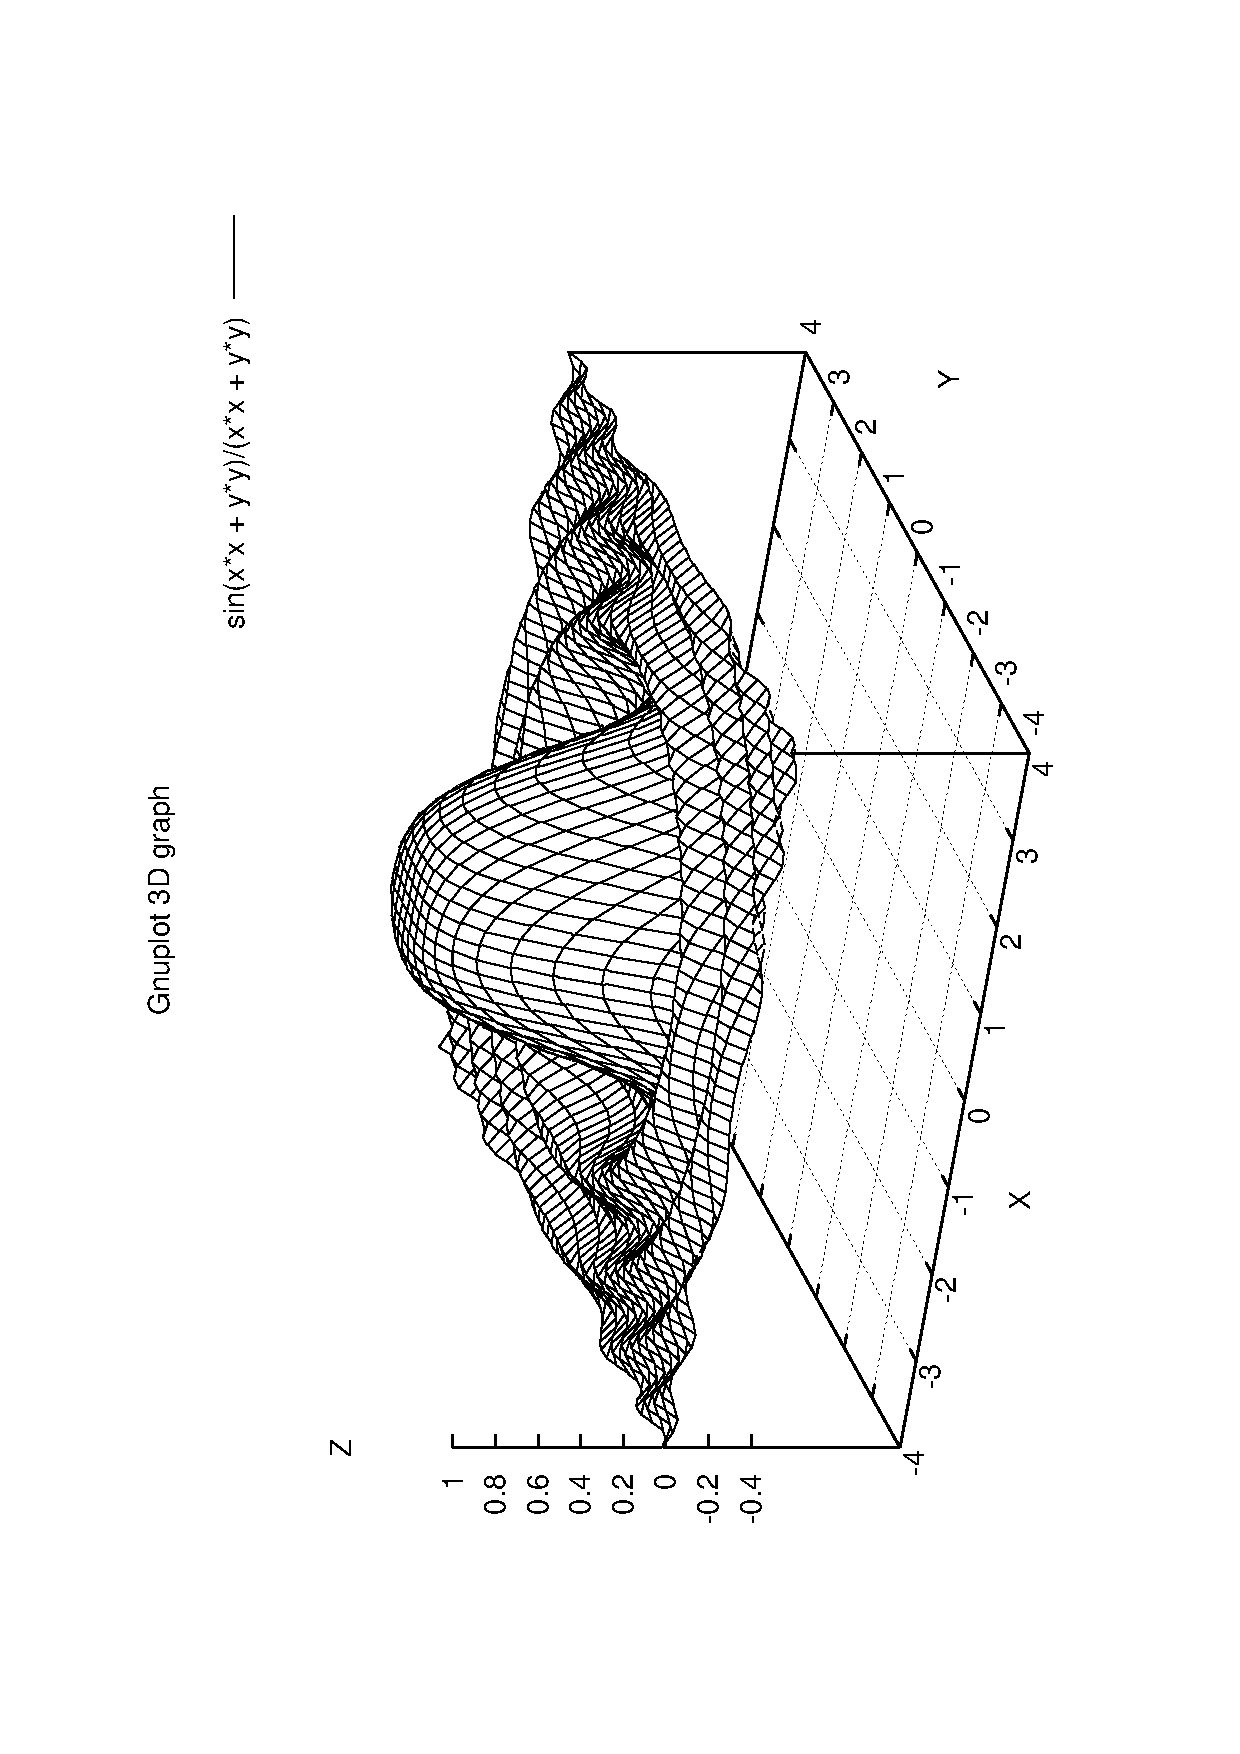
\includegraphics[width=0.6\textwidth, angle=-90]{gnuplot.pdf}}
    \caption{A Gnuplot graph.}
    \label{fig:gnuplot}
    \end{center}
  \end{minipage}
\end{figure}

When you typeset your document with \cmd{latex} then \app{dvips},
graphic inclusion only works with \texttt{EPS} files; \app{pdflatex}
accepts JPG, PNG, and of course PDF files. The latter choice might be
preferable for most users.

There are several packages that convert common graphic formats like
\file{.jpg}, \file{.gif}, \file{.png} etc. to \file{.eps} and/or
\file{.pdf}; for example, ImageMagik (\url{http://www.imagemagik.org})
and The GIMP (\url{http://www.gimp.org}). However, these applications
produce huge \PS{} files.

Best results are obtained using applications that wrap the bitmap,
turning it into a compact \PS{} file. You'll want to use \app{jpeg2ps}
(\url{http://www.pdflib.com/jpeg2ps/index.html}) or \app{bmeps}
(\href{http://www.ctan.org/tex-archive/support/bmeps}
{CTAN://support/bmeps}). The former is often the best choice for
wrapping \file{.jpg} files, but the latter handles more graphics
formats.

If you wish to make both \file{.pdf} and \file{.ps} from the same
source file, include these commands:

\begin{Verbatim}[fontsize=\small]
\usepackage{ifpdf}
...
% include the right options
\ifpdf
  \usepackage[pdftex]{graphicx}
  \pdfcompresslevel=9
\else
  \usepackage{graphicx}
\fi
...
% include the right graphic file
\ifpdf
  \includegraphics{file.png}
\else
  \includegraphics{file.eps}
\fi
\end{Verbatim}

\begin{warn}

  If you have more than 18 figures without text between them, you'll
  get the `Too many unprocessed floats' \LaTeX{} error. The quickest
  way to solve this problem is to put \cmd{clearpage} after three or
  four figures.

\end{warn}

% -----

\subsubsection{Wrapping Floats}

For a magazine-like layout, use the \package{wrapfig} package:

\begin{example}
If you meet this guy, give him some money.

\begin{wrapfigure}[4]{l}[5pt]{2cm}
{\Huge
 \texttt{=8-)}
}
\end{wrapfigure}

The reason may not be apparent to you,
but I can assure that your money
will end up in good hands.
I say again, if you meet this guy,
give him some money: he knows how to
use it properly. OK?
\end{example}

The parameters are the number of lines to be narrowed, the figure
placement, the overhang, and the figure width.

% -----

% INSERT/SHAPES

\subsection{\entry{Insert}{Shapes}}

\LaTeX{} provides a \env{picture} environment whithin which you use
commands like \cmd{circle}, \cmd{oval} and so on. In my opinion,
drawing pictures without a graphical environment is just too hard, and
\env{picture} has several limitations too. It's much better to use a
couple of great programs, both free and open source: the vector
drawing program Inkscape, \url{https://inkscape.org/}, along with
Pstoedit, \url{http://www.pstoedit.net/}.

Start Inkscape and draw any shape you wish using its tools. To insert
text rendered by \LaTeX, select \menu{Extensions/Render/LaTeX
formula...}, insert your text as in fig.~\ref{fig:ink1}, then click on
Apply.

\begin{figure}[htbp]
  \centering
  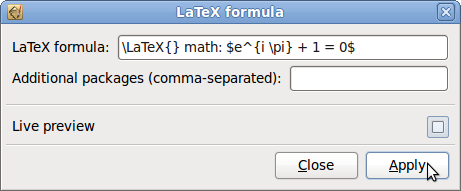
\includegraphics[width=0.6\textwidth]{inkscape-tb.png}
  \caption{Inserting a \LaTeX{} formula.}
  \label{fig:ink1}
\end{figure}

Your \LaTeX-rendered text will be included as a graphics object, and
you'll be able to edit it as you wish. The resulting picture can be
exported to several formats supported by \LaTeX, such as PDF, PNG, and
many others. More information here:
\url{http://www.ctan.org/tex-archive/info/svg-inkscape}.

\begin{figure}[htbp]
  \centering
  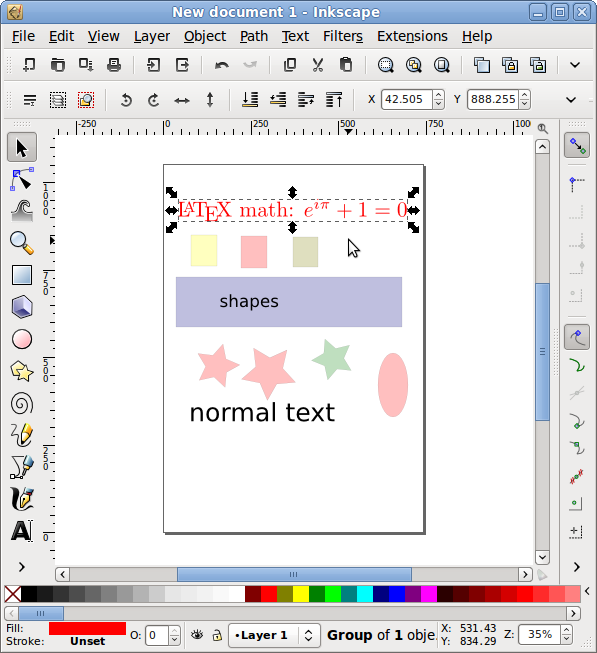
\includegraphics[width=0.6\textwidth]{inkscape.png}
  \caption{A \LaTeX{} object can be edited as desired.}
  \label{fig:ink2}
\end{figure}

If you wish to do real magic, then check out the following
packages/programs:

\begin{itemize}
  
  \item \package{pgf} is a \TeX{} macro package for generating
  graphics:\\
  \url{http://sourceforge.net/projects/pgf/}
  
  \item \package{GLE} (Graphics Layout Engine) is a graphics
  scripting language designed for creating publication quality graphs,
  plots, diagrams, figures and slides:\\
  \url{www.gle-graphics.org}
  
  \item Asymptote is a powerful descriptive vector graphics language
  that provides a natural coordinate-based framework for technical
  drawing:\\
  \url{http://asymptote.sourceforge.net/}
  
  \item ePiX, a collection of batch utilities for GNU/Linux and
  similar platforms, creates mathematically accurate figures, plots,
  and movies using easy-to-learn syntax:\\
  \url{http://mathcs.holycross.edu/~ahwang/current/ePiX.html};
  
  \item \package{pstricks} is a set of macros that allow the inclusion
  of PostScript drawings in \LaTeX{} documents:\\
  \url{http://tug.org/PSTricks/main.cgi/}
  
\end{itemize}

These packages let you make publication-quality \PS{} drawings in
\LaTeX. Many more are available; search the web for ``LaTeX vector
graphics''.

Many more kinds of `shapes' can also be inserted. To whet your
appetite, please visit the \TeX{} Showcase page,
\url{http://www.tug.org/texshowcase/}.

% -----

% INSERT/LINE

\subsection{\entry{Insert}{Line}}

Draw lines of any length and thickness with \cmd{rule}:

\begin{example}
This is a page-wide
rule:\\
\rule{\linewidth}{1pt}
but this one is shorter
and thicker:\\
\rule{2cm}{2mm}
\end{example}

Another interesting `line' is that made of dots (\cmd{dotfill}), often
used to relate things. This is how it's done:

\begin{example}
Total price \dotfill \euro~10
\end{example}

% -----

% INSERT/HYPERLINK

\subsection{\entry{Insert}{Hyperlink}}
\label{sec:hyperlink}

The \package{hyperref} package lets you write URLs and other external
references. When used together with \app{dvipdf} or \app{pdflatex},
\package{hyperref} lets you make browseable \file{.pdf} documents! For
instance, this document uses this declaration:

\begin{Verbatim}[fontsize=\small]
\usepackage[colorlinks,
            urlcolor=blue,
	    filecolor=magenta,
	    linkcolor=darkred,
	    hyperfootnotes=false]{hyperref}
\end{Verbatim}

Let's see an example:

\begin{example}
The \hypertarget{ctan}{CTAN} main site
is \url{http://www.ctan.org}, a.k.a
\href{http://www.ctan.org}{CTAN://}.

Listen to \href{run:midifile.mid}
{this MIDI file}.

Click \hyperlink{ctan}{here} to go
back to the top.
\end{example}

As you can see, the \cmd{url} command typesets its contents using a
monospace font. To use the same font as the remaining text, use the
command:

\begin{Verbatim}
\urlstyle{same}
\end{Verbatim}

after the \cmd{hyperref} declaration.

The \cmd{hypertarget} and \cmd{hyperlink} commands provide internal
links, just like HTML; \cmd{href} creates links to URLs or external
files. Note the \texttt{run:} parameter: you can run external programs
like multimedia players, office applications, whatever. As far as I
know, this feature only works in Adobe Reader, Okular, and Evince.

On Linux and possibly other \unix{} variants, you'll have to instruct
your favourite PDF reader what to run when an external file is
referenced. Insert lines like the following in your \file{.mailcap} or
\file{/etc/mailcap}:

\begin{verbatim}
audio/midi;/usr/bin/timidity %s
audio/*; xmms %s
video/*; xine -pfhq %s
\end{verbatim}

Please read \package{hyperref}'s documentation for further examples
and possibilities.

% -----

% INSERT/COMMENT

\subsection{\entry{Insert}{Comment}}

This is done inserting \% before each line, or by using the package
\package{comment} that provides the environment of the same name.

% -----

% FORMAT

\section{The \menu{Format} Menu}

In general, the main format properties of a document are set with
parame\-ters in \cmd{document\-class}: default font size (10, 11, or
12pt), paper (\texttt{a4paper}, \texttt{a5paper}, \texttt{b5paper},
\texttt{letterpaper}, \texttt{legalpaper}, \texttt{executivepaper}),
and orientation (\texttt{portrait}, \texttt{landscape}). For example, 

\begin{Verbatim}[fontsize=\small]
\documentclass[a5paper,landscape,12pt]{article}
\end{Verbatim}

Alternative font sizes can be specified as explained in
Section~\ref{sec:extsizes}.

% -----

% FORMAT/LINE SPACING

\subsection{\entry{Format}{Line Spacing}}

The package \package{setspace} provide the environments
\env{singlespace}, \env{onehalfspace}, and \env{double\-space}. In
addition, the environment/command \cmd{spacing}\cmdparm{\{amount\}}
will set the spacing to the specified amount:

\begin{example}
\begin{spacing}{2.5}
These two lines \\
are crazily spaced!
\end{spacing}
\begin{spacing}{1}
Much better, these lines\\
have a pretty space.
\end{spacing}
\end{example}

To apply line spacing to the whole document, use the
\cmd{linespread\{factor\}} command in the preamble. Default value of
\texttt{factor} is 1; larger values give larger line spacing (1.6 is
roughly double line spacing).

% -----

% FORMAT/CHARACTER

\subsection{\entry{Format}{Character}}

Standard character properties are listed in
Table~\ref{tab:properties}, font sizes in Table~\ref{tab:font_sizes}.
Please note that actual font size depends on the default size defined
in \ltx{docu\-ment\-class} (10, 11, or 12 pt); see
Table~\ref{tab:font_sizes2}.

\begin{table}[htbp]
\begin{center}
\begin{tabular}{lll} \hline
\textbf{Text attribute} & \textbf{Environment form} & \textbf{Example} \\
\hline
\cmd{textnormal} & \verb|textnormal| & main document font \\
\cmd{textrm} & \verb|rmfamily| & \textrm{roman} \\
\cmd{textit} & \verb|itshape| & \textit{italics} \\
\cmd{emph} & n/a & \emph{emphasis} \\
\cmd{textmd} & \verb|mdseries| & \textmd{medium weight (default)} \\
\cmd{textbf} & \verb|bfseries| & \textbf{boldface} \\
\cmd{textup} & \verb|upshape| & \textup{upright (default)} \\
\cmd{textsl} & \verb|slshape| & \textsl{slanted} \\
\cmd{textsf} & \verb|sffamily| & \textsf{sans serif} \\
\cmd{textsc} & \verb|scshape| & \textsc{small caps} \\
\cmd{texttt} & \verb|ttfamily| & \texttt{typewriter} \\
\cmd{underline} & \verb|underline| & \underline{underline} \\
\cmd{textsuperscript} & n/a & this is \textsuperscript{superscript} \\
\cmd{mathrm} & n/a & $\mathrm{x^n + y^n \neq z^n \forall n \neq 2}$ \\
\cmd{mathbf} & n/a & $\mathbf{x^n + y^n \neq z^n \forall n \neq 2}$ \\
\cmd{mathsf} & n/a & $\mathsf{x^n + y^n \neq z^n \forall n \neq 2}$ \\
\cmd{mathtt} & n/a & $\mathtt{x^n + y^n \neq z^n \forall n \neq 2}$ \\
\cmd{mathit} & n/a & $\mathit{x^n + y^n \neq z^n \forall n \neq 2}$ \\
\cmd{mathnormal} & n/a & $\mathnormal{x^n + y^n \neq z^n \forall n \neq 2}$ \\
\cmd{mathcal} & n/a & $\mathcal{x^n + y^n \neq z^n \forall n \neq 2}$ \\
\hline
\end{tabular}
\caption{Font attributes.}
\label{tab:properties}
\end{center}
\end{table}

Please note the difference between italics and emphasised text.
\textit{For example, this portion of text is typeset in italics, and
\emph{these words} are emphasised in upright}. As you can see,
\cmd{emph} is a \emph{logical} rather than typographic command.

Also, please note that subscript is normally used in math mode only.
The trick to use it in normal text is:

\begin{example}
this is 
$_{\mbox{\footnotesize{subscript}}}$
\end{example}

\begin{table}[ht]
\begin{center}
\begin{tabular}{ll} \hline
\textbf{Font size} & \textbf{Example} \\
\hline
\verb|tiny| & \tiny{sample text} \\
\verb|scriptsize| & \scriptsize{sample text} \\
\verb|footnotesize| & \footnotesize{sample text} \\
\verb|small| & \small{sample text} \\
\verb|normalsize| & \normalsize{sample text} \\
\verb|large| & \large{sample text} \\
\verb|Large| & \Large{sample text} \\
\verb|LARGE| & \LARGE{sample text} \\
\verb|huge| & \huge{sample text} \\
\verb|Huge| & \Huge{sample text} \\
\hline
\end{tabular}
\caption{Font sizes}
\label{tab:font_sizes}
\end{center}
\end{table}

\begin{table}[ht]
\begin{center}
  \begin{tabular}{llll}
  \hline
  Default font size & 10pt & 11pt & 12pt \\
  \hline
  \ltx{tiny} & 5 & 6 & 6 \\
  \ltx{scriptsize} & 7 & 8 & 8 \\
  \ltx{footnotesize} & 8 & 9 & 10 \\
  \ltx{small} & 9 & 10 & 10.95 \\
  \ltx{normalsize} & 10 & 10.95 & 12 \\
  \ltx{large} & 12 & 12 & 14.4 \\
  \ltx{Large} & 14.4 & 14.4 & 17.28 \\
  \ltx{LARGE} & 17.2 & 17.28 & 20.74 \\
  \ltx{huge} & 20.7 & 20.74 & 24.88 \\
  \ltx{Huge} & 24.8 & 24.88 &  24.88 \\
  \hline
  \end{tabular}
  \caption{Actual font size in pt}
  \label{tab:font_sizes2}
\end{center}
\end{table}

% -----

\subsubsection{Superscript and Subscript in Chemical Formulae}

Most chemical formulae could be entered as math formulae, using
\verb|^| and \verb|_| to obtain superscript and subscript. The
\env{mhchem} package provides a simpler command, though. Digits are
printed as subscripts by default, as superscript when preceded by
\verb|^|. Formulae must be enclosed in the \cmd{ce} command:

\begin{example}
\ce{H2O + CO2 -> H2CO3}\\
\ce{CaCO3 -> Ca^2+ + CO3^2-}\\
\ce{CO3^2- + H2CO3 -> 2 HCO3^-}\\
\ce{CaCO3 + H2CO3 -> Ca^2+ + 2HCO3^-}
\end{example}

% -----

\subsubsection{Underline styles}

Normally, \uline{underline} is not used. It's just a relic of the old
teletype era, and it doesn't look really good. If you still want to
use underline, the \package{ulem} package provides some fancy styles:

\begin{example}
\uline{important}
\uuline{urgent}
\uwave{boat}
\sout{wrong}
\xout{removed}
\end{example}

Beware: \package{ulem} redefines the \cmd{emph} command, which will be
replaced by underline. To avoid this behaviour, use this declaration:

\begin{verbatim}
\usepackage[normalem]{ulem}
\end{verbatim}


% -----

% FORMAT/CHARACTER SIZE

\subsubsection{\entry{Format}{Character Size}}
\label{sec:extsizes}

If the standard font sizes aren't enough for you, the package
\package{extsizes} may be handy. It provides `extended' versions of
the standard document classes, with support for sizes 8--12, 14, 17,
and 20 pt.

For example, let's suppose you want to typeset an article using a 17
pt font. You'll use this document preamble:

\begin{Verbatim}[fontsize=\small]
\documentclass[17pt]{extarticle}
\end{Verbatim}

Another way to get big fonts is to use the package \package{type1cm},
which provides commands like the following:

\begin{Verbatim}[fontsize=\small]
\fontsize{72pt}{72pt}\selectfont
No Smoking
\end{Verbatim}

(The example above is way too large to fit on this page{\ldots})

Parameters are font size and baseline. Yet another approach is this:

\begin{example}
\resizebox{!}{1cm}{1-cm tall}
\end{example}

\lettrine{D}{ropped} capitals at the start of a paragraph can be
obtained using the \package{lettrine} package, which provides a fully
customisable \cmd{lettrine} command. This paragraph uses the default
behaviour:

\begin{verbatim}
\lettrine{D}{ropped} capitals at the start...
\end{verbatim}

% -----


% FORMAT/FONT

\subsubsection{\entry{Format}{Character Font}}

\LaTeX{} uses its own fonts (Computer Modern), automatically generated
when needed by the \MF{} subsystem. This ensures portability and
yields very good results. However, many of us are accustomed to other
fonts: Times, Helvetica, Sans Serif{\ldots}

Fortunately, \LaTeX{} can use \PS{} fonts. Try using one of the
following packages: \package{avant}, \package{avangar},
\package{bookman}, \package{chancery}, \package{charter},
\package{courier}, \package{helvet}, \package{helvetic},
\package{ncntrsbk}, \package{newcent}, \package{palatcm},
\package{palatino}, \package{pifont}, \package{times},
\package{utopia}, \package{zapfchan}. Insert \verb|\usepackage{times}|
and enjoy the results. The only caveat is that \LaTeX{} handles maths
at its best only with Computer Modern fonts: using \PS{} fonts might
render your formulas slightly less appealing.

The packages above set the font for the whole document. To use a \PS{}
font for a region of text only, specify the font family as in the
example below. Common font families are listed in
Table~\ref{tab:font_families}. 

\begin{warn}
  Beware, some font shapes may be unavailable on some systems!
\end{warn}

\begin{example}
This is Computer Modern Roman,
{\fontfamily{phv}\selectfont
this is Helvetica!}
\end{example}

\begin{table}
\begin{center}
  \begin{tabular}{ll}
  \hline
  \textmd{Family} & \textmd{Name}\\
  \hline
  \texttt{cmr} & Computer Modern Roman\\
  \texttt{cmss} &
  {\fontfamily{cmss}\selectfont Computer Modern Sans Serif}\\
  \texttt{cmtt} &
  {\fontfamily{cmtt}\selectfont Computer Modern Typewriter}\\
  \texttt{pag} &
  {\fontfamily{pag}\selectfont Avantgarde}\\
  \texttt{pbk} &
  {\fontfamily{pbk}\selectfont Bookman}\\
  \texttt{phv} &
  {\fontfamily{phv}\selectfont Helvetica}\\
  \texttt{pnc} &
  {\fontfamily{pnc}\selectfont New Century Schoolbook}\\
  \texttt{ppl} &
  {\fontfamily{ppl}\selectfont Palatino}\\
  \texttt{ptm} &
  {\fontfamily{ptm}\selectfont Times}\\
  \texttt{pcr} &
  {\fontfamily{pcr}\selectfont Courier}\\
  \hline
  \end{tabular}
  \caption{Common font families.}
  \label{tab:font_families}
\end{center}
\end{table}

\medskip

Yet another possibility is replacing a standard \LaTeX{} font with a
\PS{} one: for example, you may want to use Avantgarde whenever
Computer Modern Sans Serif would appear. These commands can be renewed
as in the example below:

\begin{itemize}

  \item \verb|\rmdefault| (roman)
  \item \verb|\sfdefault| (sans serif)
  \item \verb|\ttdefault| (typewriter)
  \item \verb|\bfdefault| (boldface)
  \item \verb|\mddefault| (medium)
  \item \verb|\itdefault| (italics)
  \item \verb|\sldefault| (slanted)
  \item \verb|\scdefault| (small caps)
  \item \verb|\updefault| (upright)

\end{itemize}

\begin{Verbatim}[fontsize=\small]
 % Avantgarde replaces sans serif
\renewcommand{\sfdefault}{pag}
\end{Verbatim}

% -----

% FORMAT/COLOUR

\subsubsection{\entry{Format}{Character Colour}}
\label{sec:charcol}

You can colour words using the package \package{color} and appropriate
commands. Predefined colours are black, white, red, green, blue, cyan,
magenta, and yellow; you can also define your own.

\begin{example}
\textcolor{red}{This is red.}\\
\color{blue}
This text is blue!\\
So is this. Let's change.\\
\definecolor{mygreen}
{rgb}{0.1,1,0.1}
\color{mygreen}
This is my shade of green!\\
\color{black}
\colorbox{cyan}{A cyan box}\\
\fcolorbox{blue}{green}
{A green box in a blue frame}
\end{example}

Moreover, the command \cmd{pagecolor} lets you specify{\ldots} guess
what?

% -----

% FORMAT/PARAGRAPH

\subsection{\entry{Format}{Paragraph}}

Let's remind what a paragraph is according to \LaTeX: a portion of
text that either ends with \verb|\\|, or is followed by a blank line.

\emph{Environments} are \LaTeX{}'s way of specifying properties like
text alignment or font selection for a given portion of text. It's
like selecting text with the mouse, then choosing the property you
wish from a menu or clicking on a button. Another way is to enclose
the text between brackets.

Environments have this general form:

\begin{Verbatim}[fontsize=\small]
\begin{environment}
...text goes here...
\end{environment}
\end{Verbatim}

For example, if you want to center a paragraph you'll use the
\env{center} environment:

\begin{example}
\begin{center}
this text is centered
\end{center}
\end{example}

Standard environments are listed in Table~\ref{tab:environments}. In the
following sections, I'll show you what to use and when.

\begin{table}[p]
\begin{center}
\begin{tabular}{ll} \hline
\textbf{Environment} & \textbf{Purpose} \\
\hline
\ltx{abstract} & abstract\\
\ltx{array} & Math arrays\\
\ltx{center} & Centered lines\\
\ltx{description} & Labelled lists\\
\ltx{displaymath} & Formulas on their own line\\
\ltx{document} & Encloses the whole document\\
\ltx{enumerate} & Numbered lists\\
\ltx{eqnarray} & Sequence of aligned equations\\
\ltx{equation} & Displayed equation\\
\ltx{figure} & Floating figures\\
\ltx{flushleft} & Flushed left lines\\
\ltx{flushright} & Flushed right lines\\
\ltx{itemize} & Bulleted lists\\
\ltx{letter} & Letters\\
\ltx{list} & Generic list environment\\
\ltx{math} & In-line math\\
\ltx{minipage} & Miniature page\\
\ltx{picture} & Picture with text, arrows, lines and circles\\
\ltx{quotation} & Indented environment with paragraph indentation\\
\ltx{quote} & Indented environment with no paragraph indentation\\
\ltx{tabbing} & Align text arbitrarily\\
\ltx{table} & Floating tables\\
\ltx{tabular} & Align text in columns\\
\ltx{thebibliography} & Bibliography or reference list\\
\ltx{theorem} & Theorems, lemmas, etc\\
\ltx{titlepage} & For hand crafted title pages\\
\ltx{verbatim} & Simulating typed input\\
\ltx{verse} & For poetry and other things\\
\hline
\end{tabular}
\caption{Standard \LaTeX{} environments.}
\label{tab:environments}
\end{center}
\end{table}

% -----

% FORMAT/PARAGRAPH HORIZONTAL ALIGNMENT

\subsubsection{\entry{Paragraph}{Horizontal Alignment}}

By default, the text is justified. To get left--aligned,
right--aligned or centered text, use the \env{flushleft},
\env{flushright} and \env{center} environments. The commands
\cmd{raggedright}, \cmd{ragged\-left}, and \cmd{centering} are
equivalent to their correspondent environments, but they do not start
a new paragraph.

% -----

% FORMAT/PARAGRAPH VERTICAL ALIGNMENT

\subsubsection{\entry{Paragraph}{Vertical Alignment}}

The way paragraphs are separated is often puzzling to word processor
users.  \emph{Empty lines and multiple spaces are treated like a
single empty line or space}. This means that you can't get more space
between paragraphs inserting more empty lines. The commands
\cmd{smallskip}, \cmd{medskip}, and \cmd{bigskip} provide some space
between paragraphs.

If you need more space, use the command
\cmd{vskip}\{\textit{parameter}\} as in this example:

% \begin{margins}{-1cm}{-0.5cm}
\begin{example}
These paragraphs will be
separated by 1.3 cm:\\
\vskip 1.3cm
there is a 1.3 cm gap above me.
\end{example}

Note that \cmd{vskip} only works between paragraphs. What if you
wanted to start a page after an additional margin of, say, 1.5 cm?
You'll have to use \cmd{null}, which sets a `mark' in the text:

\begin{example}
\null
\vskip 1.3 cm
This text comes after 1.3 cm...
\end{example}

Finally, the command \cmd{vfill} is used to add empty lines between
two paragraphs so that the second paragraph goes exactly to the bottom
of the page. For example, 

% \begin{example} will not work here
\medskip

\begin{minipage}[c]{0.49\textwidth}
  \begin{Verbatim}[fontsize=\small]
  This appears at the top of 
  the page{\ldots}
  \vfill
  {\ldots}and this at the bottom.
  \end{Verbatim}
\end{minipage}
\begin{boxedminipage}[c]{0.49\textwidth}
  This appears at the top of
  the page{\ldots}
  \vskip 1.3 cm
  {\ldots}and this at the bottom.
\end{boxedminipage}

% -----

% FORMAT/PARAGRAPH MARGINS

\subsubsection{\entry{Paragraph}{Margins}}

Normally, the margins are set for the whole document as seen in
Section~\ref{sec:pagesetup}. Redefining them for a section of text
will not work: if you want to set a paragraph's margins, you'll have
to create a new environment like in the following example:

\begin{Verbatim}[fontsize=\small]
\newenvironment{margins}[2]
{ 
  \begin{list}{} {
    \setlength{\leftmargin}{#1}
    \setlength{\rightmargin}{#2}
  } \item }
{\end{list}}
\end{Verbatim}

Then you will use the new environment:

\begin{example}
As you can see, this paragraph
has normal margins.
\begin{margins}{0.5cm}{1cm}
 But please note that this
 paragraph has custom margins. 
\end{margins}
\end{example}

% -----

% FORMAT/PARAGRAPH INDENTATION

\subsubsection{\entry{Paragraph}{Indentation}}

To set the amount of indentation of the first line of a paragraph, we
redefine the value of the \cmd{parindent} counter. In the following
example, we set a 1-cm indentation:

\begin{Verbatim}[fontsize=\small]
\setlength{\parindent}{1cm}
\end{Verbatim}

The commands \cmd{indent} and \cmd{noindent} allow/disallow
indentation on the following paragraph. Finally, the distance between
paragraphs is set by the \cmd{parskip} counter:

\begin{Verbatim}[fontsize=\small]
\setlength{\parskip}{3pt}
\end{Verbatim}

% -----

% FORMAT/BORDER

\subsubsection{\entry{Paragraph}{Border and Shade}}

To get framed (bordered) paragraphs or words, you have the choice of
using the \package{framed} package or the \cmd{parbox} command. The
package \package{calc} is required in the latter case.

This is the simplest method, using \package{framed}:

% \begin{example} will not work here
\medskip

\begin{minipage}[c]{0.5\textwidth}
  \begin{Verbatim}[fontsize=\small]
  \setlength{\FrameRule}{2pt}
  \setlength{\FrameSep}{5pt}
  \begin{framed}
    this is a framed paragraph!
  \end{framed}
  \definecolor{shadecolor}{rgb}
  {0.9,0.8,1}
  \begin{shaded}
    this is a shaded paragraph,
    do you like it?
  \end{shaded}
  \end{Verbatim}
\end{minipage}%
\begin{minipage}[c]{0.5\textwidth}
\setlength{\FrameRule}{2pt}
\setlength{\FrameSep}{5pt}
\begin{framed}
  this is a framed paragraph!
\end{framed}
\definecolor{shadecolor}{rgb}
  {0.9,1,1}
  \begin{shaded}
    this is a shaded paragraph,
    do you like it?
  \end{shaded}
\end{minipage}

\medskip

Equivalently, use the \package{boxedminipage} package and the equally
named environment. For those who want to know more: the commands

\begin{Verbatim}[fontsize=\small]
\framebox{
  \begin{minipage}[c]{\linewidth}
  text to be framed
  \end{minipage}
}
\end{Verbatim}

are functionally equivalent to the \env{boxedminipage} environment.

% This example uses \cmd{parbox}:

% \begin{example}
% \noindent
% \fbox{
%   \parbox{\linewidth 
%     -2 \fboxsep -2 \fboxrule}
%   {again, a framed paragraph!}
% }
% \end{example}

\cmd{width} sets the width of the minipage equal to that of the
remaining text. Obviously, you can specify the width as you like.

Finally, to frame something adapting the frame to the width of the
text:

\begin{example}
this is a 
\framebox[\width]{framed}
word
\end{example}

Modifying the parameter, you can adjust the frame width:

\begin{example}
this is another
\framebox[2\width][r]{framed}
word
\end{example}

Note that the second optional parameter specifies the alignment (to
the right in this example).

% -----

% FORMAT/COLOUR

\subsubsection{\entry{Paragraph}{Colour}}

Now that you have a bordered paragraph, you'll want to set its colour
too. Do this:

\begin{example}
\colorbox{yellow}{
  \begin{minipage}
  {0.8\linewidth}
  I am a minipage, my colour
  is yellow!
  \end{minipage}
}
\end{example}

Just as an example, we set the minipage colour for only the 80\% of
its width. More about colours in Section~\ref{sec:charcol}.

% -----

% FORMAT/COLUMNS

\subsubsection{\entry{Format}{Columns}}

The commands \cmd{twocolumn} and \cmd{onecolumn} start a new page and
set the number of columns; they can also be used as parameters in
\cmd{documentclass}. If this is not enough for you, the package 
\package{multicols} provides an environment of the same name. I could
have set this section in two columns with these commands:

\begin{Verbatim}[fontsize=\small]
\columnseprule=1pt
\begin{multicols}{2}[\subsection{\entry{Format}{Columns}}]
The commands \cmd{twocolumn} ...
\end{multicols}
\end{Verbatim}

The space between columns is controlled by the parameter
\cmd{columnsep}, and the thickness of the rule between columns by
\cmd{columnseprule}. The text given as optional parameter in brackets
is excluded from the environment.

% -----

% TABLE

\section{The \menu{Table} Menu}

Quite a complex subject{\ldots} A \emph{table} is a float (as
explained in Section~\ref{sec:figure}) that must fit on one page. It
usually contains a \env{tabular} environment, even though other
possibilities exist. By default, a table adjusts its width to match
the width of its contents.

Let me stress that the \env{table} environment is a float, but
\env{tabular} is not. Keep this in mind if you want to write informal
tabular material, i.e. without label and caption.

This is the general format of a table:

\begin{Verbatim}[fontsize=\footnotesize]
\begin{table}[htbp] % placement: here, top, bottom, separate page
% \begin{small}     % sets the table font
\begin{center}      % optional
% 4-column table; alignment is left, centered, right, fixed width
\begin{tabular}{|l|c|rp{4cm}|} 
\hline              % horizontal line
\textbf{Left} & \textbf{Centre} & \textbf{Right} & \textbf{4 cm}\\
\hline
row 1, col 1 & row 1, col 2 & row 1, col 3 & row 1, col 4\\
\cline{1-2}         % horizontal line spanning columns 1-2
row 2, col 1 & row 2, col 2 & row 2, col 3 & row 2, col 4\\
\cline{1-2}
\multicolumn{2}{|c|}{spanning two columns} & row 3, col 3 & 
row 3, col 4\\
\cline{1-3}
row 4, col 1 & row 4, col 2 & row 4, col 3 & ~ \hfill right\\
% force a space with "\ "
row 5, col 1 & row 5, col 2 & row 5, col 3 & left \hfill ~\\
row 5, col 1 & row 5, col 2 & row 5, col 3 & 
~ \hfill centre \hfill ~\\
\hline
\end{tabular}
\caption{A sample table.}
% labels are used for cross references;
% for example, "see Table~\ref{tab:sampletab}"
\label{tab:sampletab}
\end{center}
% \end{small}
\end{table}
\end{Verbatim}

Table~\ref{tab:sampletab} shows the result.

\begin{table}[htbp] % placement: here, top, bottom, separate page
% \begin{tiny}
\begin{center}      % optional
% 4-column table; alignment is left, centered, right, fixed width
\begin{tabular}{|l|c|rp{4cm}|} 
\hline              % horizontal line
\textbf{Left} & \textbf{Centre} & \textbf{Right} & \textbf{4 cm}\\
\hline
row 1, col 1 & row 1, col 2 & row 1, col 3 & row 1, col 4\\
\cline{1-2}         % horizontal line spanning columns 1-2
row 2, col 1 & row 2, col 2 & row 2, col 3 & row 2, col 4\\
\cline{1-2}
\multicolumn{2}{|c|}{spanning two columns} & row 3, col 3 & 
row 3, col 4\\
\cline{1-3}
row 4, col 1 & row 4, col 2 & row 4, col 3 & ~ \hfill right\\
% force a space with "\ "
row 5, col 1 & row 5, col 2 & row 5, col 3 & left \hfill ~\\
row 5, col 1 & row 5, col 2 & row 5, col 3 & 
~ \hfill centre \hfill ~\\
\hline
\end{tabular}
\caption{A sample table.}
% labels are used for cross references;
% for example, "see Table~\ref{tab:sampletab}"
\label{tab:sampletab}
\end{center}
% \end{small}
\end{table}

Sometimes, a table is too wide and won't fit on the page. In that
case, the \package{rotating} package provides the new environment
\env{sidewaystable}. Also, \package{rotating} makes it possible to
rotate the contents of a cell by a specified angle. Finally, the
\package{tabularx} package lets one specify tables of fixed width: the
\texttt{X} column specifier indicates that a column can be spread as
needed.

Here's an example:

% \begin{example} will not work here
\medskip

\begin{minipage}[c]{0.7\textwidth}
  \begin{Verbatim}[fontsize=\small]
  \begin{sidewaystable}
    \begin{tabularx}{7.5cm}{|l|X|X|}
      \hline
      \textbf{normal} & \textbf{tilted} & 
      \textbf{wider}\\
      \hline
      normal & \rotatebox{30}{I'm tilted!} & 
      I'm wider\\
      \hline
    \end{tabularx}
  \end{sidewaystable}
\end{Verbatim}
\end{minipage}%
\begin{minipage}[c]{0.3\textwidth}
% here we cheat. Tabularx won't work inside a minipage,
% so let's load the picture.
\ifpdf
  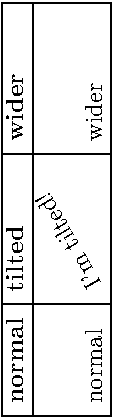
\includegraphics{tbx.pdf}
\else
  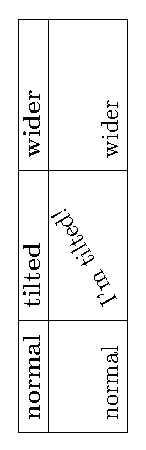
\includegraphics{tbx.eps}
\fi

\end{minipage}

\medskip

The \note standard \env{tabular} environment cannot span more than one
page! There are some packages that overcome this limitation: you will
want to try out \package{longtable}, \package{supertabular}, and
\package{xtab}.

To enable colours in tables, you use the \package{colortbl} package:

\begin{example}
Colour by row:\\\vskip 2mm
\begin{tabular}{|l|c|r|}
  \hline
  \rowcolor{cyan}
  one & two & three\\
  \rowcolor{green}
  one & two & three\\
  \rowcolor{yellow}
  one & two & three\\
  \hline
\end{tabular}
\end{example}

\begin{example}
Colour by column:\\\vskip 2mm
\begin{tabular}
  {|>{\columncolor{cyan}}l|
  >{\color{red}
  \columncolor{green}}c|
  >{\columncolor{yellow}}r|}
  \hline
  one & two & three\\
  one & two & three\\
  one & two & three\\
  \hline
\end{tabular}
\end{example}

To conclude the subject, a neat little trick. If you think that
writing \LaTeX{} tables is too complicated, you could be relieved by
OpenOffice Calc and Calc2LaTeX. The former is the well-known free
spreadsheet, while the latter is a plugin that that lets you turn a
cell range into a \LaTeX{} table. Links:
\url{http://www.openoffice.org/}, 
\url{http://calc2latex.sourceforge.net/}.


% -----

\subsection{\entry{Table}{Line Spacing}}

A line adjusts itself to the height of the text it contains. To add
some space \emph{before} a line, the trick is to start it with a
\texttt{\textbackslash{}rule} of 0 length and specified height. To add
space \emph{after} a line, use
\texttt{\textbackslash{}\textbackslash{}} followed by optional space.
Here is an example:

\begin{example}
\begin{tabular}{lll}
one & two & three\\
0.3 centimeters & \textbf{after} &
  this line\\[0.3cm]
one & two & three\\
one & two & three\\
\rule{0pt}{1.2cm}1.2 centimeters &
  \textbf{before} & this line\\
\end{tabular}
\end{example}

% -----

\subsection{\entry{Table}{Rule Width}}

% TO DO: \setlength{\arrayrulewidth}{<width>}

\begin{example}
\begin{tabular}{|lll|}
\hline
%\setlength{\arrayrulewidth}{5pt}
one & two & three\\
\hline
four & five & six\\
%\setlength{\arrayrulewidth}{1pt}
\hline
\end{tabular}
\end{example}

% -----

\subsection{\entry{Table}{Aligning Numbers}}

A special case of a tabular environment is when we want to align
numbers with respect to the decimal positions. 

The simplest method is using the \ltx{@} column specifier, which in
practice is useful in tables containing only numbers. The column
separator \texttt{\&} is replaced by the decimal dot:

\begin{example}
\begin{tabular}{r@{.}l}
 3&14159\\
 1&61803\\
 1&41421\\
 100&00000
\end{tabular}
\end{example}

Alternatively, use the \package{dcolumn} package, which adds the
\texttt{D} column specifier. \texttt{D} has three arguments: the
separator to use in the \LaTeX{} source and in output (usually the
same, `.'), and the number of digits to the right of the decimal place
indicator. Optionally, the third argument can specify the number of
digits to the left and to the right of the decimal place indicator,
separated by a dot. Lastly, if the third argument is -1, the material
of the column is centered around the separator.

All material in the table is typeset in math mode. To insert headings,
you'll have to put the text in an \cmd{mbox}.

% \begin{example} will not work here
\medskip

\begin{minipage}[c]{0.5\textwidth}
  \begin{Verbatim}[fontsize=\small]
  \begin{tabular}{|D{.}{,}{4.2}|%
  D{.}{.}{5}|D{.}{.}{-1}|}
  \hline
  \mbox{One} & \mbox{Two} &
  \mbox{Three}\\
  10.33 & 10.33 & 10.33\\
  1000 & 1000 & 1000\\
  5.1 & 5.1 & 5.1\\
  3.14 & 3.14159 & 3.14159\\
  \hline
  \end{tabular}
  \end{Verbatim}
\end{minipage}%
\begin{minipage}[c]{0.5\textwidth}
\begin{tabular}{|D{.}{,}{4.2}|%
D{.}{.}{5}|D{.}{.}{-1}|}
\hline
\mbox{One} & \mbox{Two} &
\mbox{Three}\\
10.33 & 10.33 & 10.33\\
1000 & 1000 & 1000\\
5.1 & 5.1 & 5.1\\
3.14 & 3.14159 & 3.14159\\
\hline
\end{tabular}
\end{minipage}

% -----

\subsection{Using \package{slashbox}}

This package add the \cmd{backslashbox} command:

\medskip

\begin{minipage}[c]{0.5\textwidth}
  \begin{Verbatim}[fontsize=\small]
\begin{tabular}{|l|l|l|}
  \hline
  \backslashbox[2cm]{Lesson}{Date} & 
  Monday & Tuesday\\
  \hline
  Stratigraphy & room A & room A\\
  Chemistry & room B & Lab $\alpha$\\
  Physics & room C & Lab $\beta$\\
  \hline
\end{tabular}
\end{Verbatim}
\end{minipage}%
\begin{minipage}[c]{0.5\textwidth}
\begin{tabular}{|l|l|l|}
  \hline
  \backslashbox[2cm]{Lesson}{Date} & 
  Monday & Tuesday\\
  \hline
  Stratigraphy & room A & room A\\
  Chemistry & room B & Lab $\alpha$\\
  Physics & room C & Lab $\beta$\\
  \hline
\end{tabular}
\end{minipage}

\medskip

% \emph{TODO: mention \cmd{newcolumntype} and \package{floatflt}}

% -----

\subsection{Importing Data in \LaTeX{} Tables}

For many people, data files are the bread and butter of everyday's
work. Most data files are simply ASCII text with columns of numbers,
but some people use spreadsheets. Nearly all spreadsheet applications
can export sheets in the ASCII-based \file{.csv} file format; values
are usually separated by the `;' character.

Converting a data file into a \LaTeX{} table is quite a tedious
process. The following script for \unix{} will convert a datafile with
an arbitrary number of columns to a table. It will also work on
\file{.csv} files.

\begin{Verbatim}[fontsize=\small]  
#!/bin/sh

# dat2tex.sh: converts tabular data to a tabular environment

if [ $# != 1 ]; then
  echo "Usage: $0 <datafile>"
  exit 1
fi

# is this a csv file?
grep ";" $1 > /dev/null
if [ $? = 0 ]; then
  AWK="awk -F;"
else
  AWK=awk
fi

# ok awk, make my day
$AWK '{if (1 == FNR) { \
        printf "\\begin{tabular}{"; \
        for (i = 1; i <= NF; i++) {printf "l"}; \
        printf "}\n"
      }
      for (i = 1; i < NF; i++) \
        {printf $i" & "} printf $NF"\\\\ \n"} \
      END {printf "\\end{tabular}\n"}' $1

# end of dat2tex
\end{Verbatim}

% -----

% TOOLS

\section{The \menu{Tools} Menu}

% -----

% TOOLS/MAIL MERGES

\subsection{\entry{Tools}{Mail Merges}}

This useful and time-saving tool is implemented in \LaTeX{} by the
\package{textmerg} package. Let's consider a simple document, in which
the name, surname, and title of people we're writing to may vary. The
remaining text does not change.

We'll define three \emph{fields}, which are the variable part of the
text: \cmd{Name}, \cmd{Surname}, and \cmd{Title}. Their values will be
gathered from an external file, \file{data.dat}.

\begin{Verbatim}[fontsize=\small]
\documentclass{article}
\usepackage{textmerg}
\begin{document}
% let's declare the variable fields:
% \Void is for empty lines
\Fields{\Name\Surname\Title-\Void}
\Merge{data.dat}{%
Dear \Title{} \Surname,\\
may I call you \Name?\\
Yours,\\
\hspace{3cm}Guido\clearpage}
\end{document}
\end{Verbatim}

The fourth field, \cmd{Void}, isn't really necessary and it's there
for illustration. It's preceded by a minus sign, which indicates that
it can be empty in the data file. Simply put, we want to separate the
records using empty lines.

The file \file{data.dat} reads:

\begin{Verbatim}[fontsize=\small]
Guido
Gonzato
Dr.

Francesco
Mulargia
Prof.

Marie
Curie
Mme

\end{Verbatim}

That's it: the resulting output will contain the merged text, one page
for each recipient.

% -----

% TOOLS/LABELS

\subsection{\entry{Tools}{Labels}}

If making mail merges was easy, making labels is even trivial. Let's
suppose you want to make 20 equal labels on a 3$\times$8 peel--off
label sheet. The package to use, predictably, is called
\package{labels}. In this example, we'll make 10 plain labels and 10
boxed labels:

\begin{Verbatim}[fontsize=\small]
\documentclass[a4paper,12pt]{article}
\usepackage{labels}
\LabelCols=3      % n. of columns of labels
\LabelRows=8      % n. of rows of labels
\LeftBorder=8mm   % borders of each label
\RightBorder=8mm
\TopBorder=5mm
\BottomBorder=5mm
\LabelGridtrue      % show the grid
\numberoflabels=10  % number of labels of each type to print
% the text of the label is specified by
% the \addresslabel[]{} macro:
\begin{document}
  \addresslabel[\large] % optional arguments
  {\textbf{Guido Gonzato}, Ph.D.\\
  \textsl{Linux system manager}}
  % now on to the boxed labels
  \boxedaddresslabel[\fboxsep=4mm\fboxrule=1mm]
  {\textbf{Guido Gonzato}, Ph.D.\\
  \textsl{Linux system manager}}
\end{document}
\end{Verbatim}

% You'll also have to choose the correct paper size and adjust the page
% margins (use \package{geometry}; omitted in this example).

To make labels containing different addresses, you may use either an
external file or insert the addresses in the main file:

\begin{Verbatim}[fontsize=\small]
\documentclass[a4paper,12pt]{article}
\usepackage{labels}
\LabelCols=3
\LabelRows=8
\LeftBorder=3mm
\RightBorder=3mm
\TopBorder=8mm
\BottomBorder=8mm
\LabelGridtrue
\begin{document}
% use either this environment:
\begin{labels}
  1$^{st}$ name
  1$^{st}$ address
  1$^{st}$ city, state, zipcode

  2$^{nd}$ name
  2$^{nd}$ address
  2$^{nd}$ city, state, zipcode

  3$^{rd}$ name
  3$^{rd}$ address
  3$^{rd}$ city, state, zipcode
\end{labels}
% or an external file containing exactly the same text:
% \labelfile{addresses.dat}
\end{document}
\end{Verbatim}

It is left to you to combine \package{textmerg} and \package{labels}!

% -----

% TOOLS/LANGUAGE

\subsection{\entry{Tools}{Default Language}}

\LaTeX{} default language is English, but other languages are
supported. By language support I mean the translation of terms like
`Chapter' or `Index', correct hyphenation, and the possibility of
inserting characters like `\c c' or `\'e' directly via your keyboard.
(The normal way being typing \texttt{\bs{}c c} and \texttt{\bs{}'e}.)

Your \LaTeX{} distribution contains a file called \file{language.dat}
(usually \path{$TEXMF/tex/generic/config/language.dat} that contains a
list of languages. Editing this file you choose the languages for
which you want hyphenation patterns.

If you are not a native English speaker, you'll want to use the
package \package{babel} as in the following example:

\begin{Verbatim}[fontsize=\small]
\usepackage[italian,english]{babel}
\end{Verbatim}

\begin{warn}

  \package{babel} alters the way some characters behave in a
  language-dependent way. If you experience odd problems, insert the
  offending characters using the \cmd{charXX} syntax.

\end{warn}

In addition, to type accented letters and in general non-standard
ASCII characters\footnote{in computer jargon, `standard ASCII
characters' are the characters whose code is included between 32
(space) and 126 (tilde).} you may want to use the packages
\package{inputenc} and \package{fontenc}. In most cases, UTF-8 is the
right choice: remember to enable it in your editor too!

\begin{Verbatim}[fontsize=\small]
\usepackage[utf8]{inputenc}
\usepackage[T1]{fontenc}
\end{Verbatim}

A different way of inserting accented letters is configuring your
editor to type those for you. For example, I set up my editor of
choice (\app{jed}) to have it insert \texttt{\bs{}'e} whenever I type
`\'e'. I included this in my \file{.jedrc}:

{\small
\begin{alltt}
define latex_mode_hook ()
\{
  set_abbrev_mode (1);
  if ( () = abbrev_table_p ("LaTeX") )
    use_abbrev_table ("LaTeX");
#ifdef WIN32
  % prevent clash with movement keys
  undefinekey ("\`a\`a", "LaTeX-Mode");
  definekey (" \bs\bs`a", "\`a\`a", "LaTeX-Mode");
#else
  local_setkey (" \bs\bs`a",     "\`a");
#endif
  local_setkey (" \bs\bs'e",     "\'e");
  local_setkey (" \bs\bs`e",     "\`e");
  local_setkey (" \bs\bs`\bs\bs{}i\{\}", "\`\i");
  local_setkey (" \bs\bs`o",     "\`o");
  local_setkey (" \bs\bs`u",     "\`u");
\}
\end{alltt}
}

Please consult your editor's documentation.

% -----

% TOOLS/HYPHEN

\subsection{\entry{Tools}{Hyphenation}}

Although \LaTeX{} usually does a good job at hyphenating words,
sometimes manual intervention may yield better results. Manual hyphens
are specified inserting \verb|\-| where we want the word to be broken.
A better way is to declare hyphenation rules:

\begin{Verbatim}[fontsize=\small]
\hyphenation{ge-o-phy-sics ge-o-lo-gy earth}
\end{Verbatim}

The above declaration instructs \LaTeX{} not to hyphen the word
`earth'. Another way to prevent a word to be hyphenated is to put it
in \cmd{mbox}:

\begin{Verbatim}[fontsize=\small]
Do not hyphen \mbox{internationalisation}, please. I'm a masochistic.
\end{Verbatim}

% -----

% TOOLS/SPELL CHECK

\subsection{\entry{Tools}{Spell Check}}

\LaTeX{} is not aware of spell spelling. This task is done using
external tools like \app{ispell}, \app{aspell} or others. Under \unix,
you can use \app{ispell} this way:

\begin{Verbatim}[fontsize=\small]
shell> ispell -t mydocument.tex
\end{Verbatim}

The \texttt{-t} switch instructs \app{ispell} to ignore \TeX{} and
\LaTeX{} commands. If your language is not English, specify the
appropriate dictionary with the \texttt{-d} switch:

\begin{Verbatim}[fontsize=\small]
shell> ispell -d italiano -t mydocument.tex
\end{Verbatim}

% -----

% HELP

\section{The \menu{Help} Menu}

There are many ways of getting help with \LaTeX{}, both online and offline.
The best place to start is the CTAN site,
\url{http://www.ctan.org/tex-archive/info/}.

\begin{itemize}

  \item \verb|info latex| (\unix{} systems) gives a concise but very complete
    on-line summary of commands and concepts;
    
  \item \url{http://www.ctan.org/tex-archive/info/LatexHelpBook/} is a very
    nice help system for \LaTeX{}, fully integrated with Windows.
    
  \item don't forget the
  \url{http://groups.google.com/group/comp.text.tex/topics} newsgroup:
  it's an invaluable source of help.
  
\end{itemize}

As of 2015, most GNU/Linux distributions ship with \app{TeXLive},
probably the most complete \TeX/\LaTeX{} systems. A lot of
documentation is provided; on my Ubuntu machine, it's found in
\path{/usr/share/doc/texlive-doc/}.

% -----

\section{The End}

This document is copyleft \textcopyright{} Guido Gonzato, 2001--2015,
and released under the GNU Free Documentation Licence. I really hope
you'll find this guide useful. For any suggestions or comments, please
feel free to contact me.

\newpage

% -----

\appendix

\section{Document Templates}
\label{ap:templates}

A template for the class \texttt{article} was presented in
Section~\ref{sec:filenew}. More examples are shown in the following
figures.

% -----

% BOOK

\begin{figure}[htbp]
\begin{Verbatim}[fontsize=\small]
\documentclass[twoside,11pt]{book}
\begin{document}
\frontmatter
\begin{titlepage}
\title{The Book of Mine}
\end{titlepage}
\author{John B. Smith}
\maketitle
\tableofcontents
\mainmatter
\part{The Beginning}
\chapter{Introduction}
\section{Let's Start}
The book starts here.
\part{The End}
\backmatter
Thank you for reading this book.
\end{document}
\end{Verbatim}
\caption{Book template.}
\end{figure}

% -----

% REPORT

\begin{figure}[htbp]
\begin{Verbatim}[fontsize=\small]
\documentclass[twoside,12pt]{report}
% tables and figures at the end:
\usepackage{endfloat}
\begin{document}
\title{Final Report}
\author{John B. Smith}
\date{London, \today}
\maketitle
\begin{abstract}
This is the final report.
\end{abstract}
\tableofcontents
\listoftables
\listoffigures
\part{Start}
\chapter{Begin}
\section{Introduction}
The report starts here.
\end{document}
\end{Verbatim}
\caption{Report template.}
\end{figure}

% -----

% LETTER

\begin{figure}[htbp]
\begin{Verbatim}[fontsize=\small]
\documentclass[12pt]{letter}
\begin{document}
\address{My address}
\signature{Guido}
\begin{letter}{John's address}
\opening{Dear John,}
Thank you for being my friend.
\closing{Hope to see you soon,}
\ps{P.S. Say hello to granny!}
\encl{My son's photographs!}
\end{letter}
\end{document}
\end{Verbatim}
\caption{Letter template.}
\end{figure}

% -----

% NOTICE

\begin{figure}[htbp]
\begin{Verbatim}[fontsize=\small]
\documentclass[a4paper]{article}
\usepackage{type1cm}
\usepackage{times}
\usepackage{color}
\usepackage{rotating}
\pagestyle{empty}
\begin{document}
\begin{sidewaysfigure}
  \fontsize{2.5cm}{2.5cm}\selectfont
  \centerline{\textcolor{blue}{\textbf{Please:}}}
  \vskip 1cm
  \fontsize{4cm}{3cm}\selectfont
  \centerline{\textcolor{red}{DO NOT}}
  \centerline{\textcolor{red}{SMOKE}}
  \centerline{\textcolor{red}{HERE!}}
  \vskip 1cm
  \fontsize{2cm}{2cm}\selectfont
  \centerline{\textcolor{magenta}{If you do,}}
  \centerline{\textcolor{magenta}{you'll be \emph{deboned!}}}
\end{sidewaysfigure}
\end{document}
\end{Verbatim}
\caption{How to write a notice.}
\end{figure}

% -----

% POSTER

\begin{figure}[htbp]
\begin{Verbatim}[fontsize=\small]
\documentclass{article}
\usepackage[absolute,showboxes]{textpos}
\usepackage{color}
\usepackage{framed}
\usepackage{graphicx}
\setlength{\TPHorizModule}{10mm} % standard unit of length
\setlength{\TPVertModule}{\TPHorizModule}
\setlength{\TPboxrulesize}{1pt}  % box line width
% start everything near the top-left corner
\textblockorigin{0mm}{0mm}

\begin{document}
\setlength{\parindent}{0pt}
\definecolor{shadecolor}{rgb}{0.9,1,1}
\begin{textblock}{5}(0,0)
% this block is 5 modules wide; height is
% automatically determined
\begin{center}
  \begin{minipage}[c]{0.8 \linewidth}
  \begin{shaded}
  This block is placed with its top left corner at the `origin'
  on the page, which has been set to (0mm,0mm). The internal
  margin and the shading are provided by the \texttt{minipage}
  and \texttt{shaded} environments.
  \end{shaded}
  \end{minipage}
\end{center}
\end{textblock}
\begin{textblock}{6}(10,1)
  \includegraphics[width=6cm,angle=-90]{gnuplot.ps}
  This picture is at (10,1). Note that rotating it
  by -90 makes it overflow the margin.
\end{textblock}
\begin{textblock}{5}[0.5,0.5](2.5,8)
This block is at position (2.5,8), but because the optional
argument [0.5,0.5] has been given, it is the centre of the block
which is located at that point, rather than the top-left corner.
\end{textblock}
\begin{textblock}{3,4}(6,4)
The dimensions of this block are 3$\times$4 cm.
Its origin is position (6,4) on the page. Note that the text
overflows the margin in some cases; you'll want to 
use the \texttt{minipage} environment to prevent that.
\end{textblock}
\end{document}
\end{Verbatim}
\caption{How to write a poster.}
\label{fig:poster}
\end{figure}

% -----

% The End

\end{document}
